% Monografia para Projeto de Fim de Curso - Igor Cleto Silva de Araújo
%-----------------------------------------------------------


%---------------Inicialização de pacotes--------------------

\documentclass[12pt,a4paper,notitlepage,twoside]{book}


\usepackage{graphicx}
\usepackage[utf8]{inputenc}
%\usepackage[latin1]{inputenc} %%pode ser necessário trocar a codificação em sistemas Windows
\usepackage[brazil]{babel}		%%pode ser necessário trocar o pacote de línguas em algumas distribuições LateX
%\usepackage[portuguese]{babel}
\usepackage[T1]{fontenc}
\usepackage{amsmath,amssymb}
\usepackage{amsthm,amsfonts}
\usepackage{color}
\usepackage[colorlinks]{hyperref}
\usepackage{abntex2abrev}
%\usepackage[alf]{abntex2cite} %se você quiser seguir as normas ABNT no sistema autor-data
%\usepackage[num]{abntex2cite} %se você quiser seguir as normas ABNT no sistema numérico
\usepackage{setspace}
\usepackage[toc,page]{appendix}

%Definindo fonte Times (Use os pacotes obsoletos se não conseguir instalar os atualizados)
%\usepackage{times}     %Pacote de fontes obsoleto, apenas texto
%usepackage{mathptmx}  %Pacote de fontes obsoleto, texto e símbolos matemáticos
%\usepackage{newtxtext,newtxmath}  %Pacotes de fontes mais recentes

\usepackage[a4paper,top=30mm,bottom=30mm,inner=30mm,outer=25mm,headheight=7mm,headsep=6mm,footskip=7mm]{geometry}
\usepackage{enumerate}

\makeindex

%\singlespacing   %%espaçamento simples
%\onehalfspacing
%\setstretch{1.03} %%um pouco melhor que espaçamento simples
\linespread{1.25} %corresponde ao espaçamento 1.5 do MS Word

%---------------Início do documento-------------------------

\begin{document}

\begin{titlepage}
\begin{center}
{\large Universidade Federal de Minas Gerais\\
Escola de Engenharia \\
Curso de Graduação em Engenharia de Controle e Automação\\}

\vspace{6cm}
{\bf\Large Monitoramento e previsão do consumo de energia residencial baseado em Sistemas
Inteligentes\vspace{0.2cm}}

\vspace{4cm}

%\hspace{0.3\textwidth} \parbox{0.65\textwidth}
{\large Igor Cleto Silva de Araújo}
\vspace{2cm}  
   
\vspace{2cm}          
%\hspace{0.3\textwidth} 
{\large Orientadora: Prof Carmela Maria Polito Braga}\\

\vfill
%\hspace{0.3\textwidth} 
{\large Belo Horizonte, Outubro de 2024 }
\end{center}

\end{titlepage}

\newpage
\clearpage
\thispagestyle{empty}


\begin{titlepage}

\centering
\textbf{Monografia}\\
\vspace{2cm}
\centering
\textbf{Monitoramento e previsão do consumo de energia residencial baseado em Sistemas
Inteligentes}\\
\vspace{5cm} 

\parbox{1.0\textwidth} 
{\large 
Monografia submetida à banca examinadora
designada pelo Colegiado Didático do Curso de
Graduação em Engenharia de Controle e
Automação da Universidade Federal de Minas
Gerais, como parte dos requisitos para aprovação na
atividade Projeto Final de Curso II.}

\vspace{7cm} 
\centering
Belo Horizonte, Outubro de 2024

\end{titlepage}


\pagenumbering{roman}
\addcontentsline{toc}{chapter}{Resumo}

\begin{center}
\huge{{\bf Resumo}}
\vspace{2cm}
\end{center}

No Resumo, em uma única página, em no máximo dois parágrafos, você explicita os seguintes itens: objetivos do projeto e descrição sucinta do local onde ele foi desenvolvido; metodologia utilizada; e resultados alcançados. Leitores experientes decidem se prosseguirão para a leitura do texto completo após lerem o resumo, a conclusão e a introdução. Por isso nestes lugares você deve colocar um esforço maior de convencimento. Além disso, a linguagem utilizada deve ser acessível a leitores com pouca familiaridade com a área, limitando-se o uso de jargões.
 
\begin{sloppypar}
Este novo parágrafo serve para mostrar que ao pular uma ou mais linhas no texto do arquivo .tex, o \TeX\ entende que você está iniciando outro parágrafo. O comando \textsf{sloppypar} força o texto a não ultrapassar as margens. Só deve ser usado se este problema ocorrer.
\end{sloppypar}

 
\clearpage
\thispagestyle{empty}
\cleardoublepage


\addcontentsline{toc}{chapter}{Abstract}

\begin{center}
\huge{{\bf Abstract}}
\vspace{2cm}
\end{center}

This project aims to develop an intelligent system for monitoring and forecasting energy consumption in homes that were not originally designed for home automation. Specifically, it seeks to research and analyze existing technologies that allow energy monitoring without requiring prior infrastructure, and to explore solutions suitable for conventional residences. The project will involve the development of a prototype for an easily installable and user-friendly monitoring system, as well as the implementation of data processing algorithms and consumption forecasting using artificial intelligence techniques. An intuitive software platform will be created for users to visualize and analyze the data, and the system will be tested and validated in a real-world environment to ensure its efficiency and usability. To promote the feasibility of large-scale implementation, the project will include cost analysis and strategies for adoption. Finally, the results will be documented and disseminated, emphasizing the contributions to Control and Automation Engineering and the social and environmental benefits provided by the developed system. 

\clearpage
\thispagestyle{empty}
\cleardoublepage


\addcontentsline{toc}{chapter}{Agradecimentos}

\begin{center}
\huge{{\bf Agradecimentos}}
\vspace{4cm}
\end{center}

Gostaria de expressar minha profunda gratidão a Deus, pela saúde física e mental que me permitiu a realização dos meus sonhos e objetivos. Aos meus pais, meu sincero agradecimento pelo suporte incondicional aos meus estudos desde a minha infância, sempre acreditando em meu potencial e me incentivando a seguir em frente. Agradeço também aos meus professores e gestores, que, com seu apoio e ensinamentos, tanto dentro quanto fora da sala de aula, contribuíram para a minha formação acadêmica e pessoal. Não poderia deixar de agradecer, de maneira especial, à minha orientadora, Profª. Carmela Maria Polito Braga, pela dedicação, paciência e orientação ao longo deste um ano de desenvolvimento deste trabalho. Sua contribuição foi fundamental para a realização deste projeto. A todos, meu muito obrigado.
 
\clearpage
\thispagestyle{empty}
\cleardoublepage
\tableofcontents
%\markboth{Conteúdo}{Conteúdo}

\clearpage
%\thispagestyle{empty}
%\cleardoublepage

% Normalmente, este arquivo só contém isto.
\listoffigures
\addcontentsline{toc}{chapter}{Lista de Figuras}
%\markboth{Lista de Figuras}{Lista de Figuras}

\clearpage
%\thispagestyle{empty}
%\cleardoublepage

% Normalmente, este arquivo só contém isto.
\listoftables
\addcontentsline{toc}{chapter}{Lista de Tabelas}
%\markboth{Lista de Tabelas}{Lista de Tabelas}

\clearpage
%\thispagestyle{empty}
%\cleardoublepage

% Normalmente, este arquivo só contém isto.

\pagenumbering{arabic}
\setcounter{page}{1}
\chapter{Introdução}
\label{chap:intro} %este label será usado para referenciar este capítulo

% As primeiras frases têm a missão de prender a atenção do leitor e por isso são as mais importantes do texto. Diga o quanto antes o que você fez e quais são os resultados alcançados. Ao terminar de ler a introdução o leitor tomará uma nova decisão de se vale a pena ou não continuar lendo o texto. Capte a atenção do leitor bem aqui.

% A comunicação escrita é considerada umas das cinco habilidades mais importantes por profissionais de engenharia e um engenheiro passa em média mais de $25$\% do seu tempo escrevendo \cite{eggert2002response,spretnak1982survey}. Uma quantidade similar de tempo é gasta na escrita de correspondência e de relatórios técnicos \cite{cunningham2012perceptions}. Dessa forma, encare a escrita do seu projeto como um treinamento nessa importante habilidade.

% Neste texto você encontrará não apenas uma estrutura para escrever seu trabalho em \LaTeX, mas também um pequeno manual de boas práticas na escrita técnica. Leia com atenção e coloque as sugestões em prática à medida que preenche o texto com o conteúdo do seu próprio projeto. Também será apresentado um número de vícios de escrita comumente encontrados nas monografias de alunos. 

% A seguir está a estrutura de organização sugerida pelo colegiado do curso. Note que ela não é necessariamente a melhor para contar a história do seu projeto. Você pode por exemplo preferir usar títulos mais pertinentes ao seu contexto. Contudo, o seu texto deve conter cada um dos pontos a seguir.

\section{Motivação e Justificativa}
\label{sec:motivacao}

A crescente demanda por energia elétrica, aliada à necessidade de uso eficiente dos recursos energéticos, torna imperativo o desenvolvimento de soluções inovadoras que permitam aos consumidores monitorar e gerenciar seu consumo de forma eficaz e em tempo real. No contexto residencial, muitas vezes os usuários não têm acesso a informações detalhadas sobre o consumo energético em suas casas, o que dificulta a identificação de desperdícios e a implementação de medidas para a redução do consumo. O cenário se agrava devido à falta de sistemas acessíveis e de fácil implementação para o monitoramento eficiente, o que resulta em uma grande dificuldade para os consumidores em adotar práticas mais sustentáveis e econômicas no seu cotidiano. 

Além disso, a automação residencial enfrenta desafios consideráveis relacionados à integração de dispositivos e sensores de diferentes fabricantes. A grande diversidade de tecnologias, protocolos de comunicação e padrões de mercado, somada à ausência de uma padronização efetiva entre os diferentes fabricantes, cria um ambiente no qual os dispositivos muitas vezes não se comunicam de maneira eficiente, impedindo a criação de sistemas unificados de monitoramento e controle. Esse cenário limita os benefícios da automação, como a otimização do consumo de energia e a melhoria da qualidade de vida dos moradores, além de dificultar o acesso a tecnologias que poderiam proporcionar um ambiente mais confortável, seguro e sustentável.

Adicionalmente, muitas residências não foram originalmente projetadas com infraestrutura para automação, o que torna a adaptação desses ambientes ao uso de tecnologias de monitoramento e controle mais complexa e dispendiosa. A implementação de soluções de automação, frequentemente, exige modificações estruturais significativas, que podem tornar o processo oneroso e inviável para uma grande parcela da população. Isso, por sua vez, desencoraja muitos proprietários a adotarem essas tecnologias, deixando uma significativa quantidade de residências sem os benefícios em termos de eficiência energética, conforto e segurança que poderiam ser proporcionados por sistemas de automação. Assim, a falta de alternativas acessíveis e de fácil implementação para o monitoramento e gestão do consumo energético representa uma grande oportunidade de desenvolvimento de soluções que possam superar essas barreiras técnicas e financeiras e beneficiar uma ampla gama de usuários.

\section{Objetivos do Projeto}
\label{sec:objetivos}

Tendo em vista o exposto acima, este projeto tem por objetivos:

\begin{enumerate}[a)]
\item Realizar uma pesquisa e análise de tecnologias existentes que permitam o monitoramento energético sem a necessidade de infraestrutura prévia;
\item Explorar soluções adequadas para residências convencionais, que não foram originalmente projetadas para automação residencial;
\item Desenvolver um protótipo de sistema de monitoramento de fácil instalação e uso;
\item Implementar algoritmos de processamento de dados e previsão de consumo utilizando técnicas de inteligência artificial;
\item Criar uma plataforma de software intuitiva para visualização e análise dos dados pelos usuários;
\item Testar e validar o sistema em ambiente real, garantindo sua eficiência e usabilidade;
\item Promover a viabilidade de implementação em larga escala por meio da análise de custos e estratégias de adoção;
\item Documentar e divulgar os resultados obtidos, destacando as contribuições para a Engenharia de Controle e Automação e os benefícios sociais e ambientais proporcionados pelo sistema desenvolvido.
\end{enumerate}

\section{Local de Realização}
\label{sec:empresa}

O local de realização deste projeto é a residência do próprio desenvolvedor, onde os testes dos equipamentos e a simulação das necessidades reais de automação residencial estão sendo realizados. A escolha deste ambiente se justifica pela possibilidade de realizar uma avaliação prática e realista das soluções de monitoramento e previsão de consumo energético, simulando as condições do dia a dia em uma residência convencional. A residência não foi originalmente projetada com infraestrutura para automação, o que representa um desafio adicional, mas também um aspecto relevante para a validação do sistema, pois permite testar a adaptação de tecnologias em um ambiente que não conta com recursos avançados de automação.

Neste contexto, o projeto visa avaliar a viabilidade de implementação de soluções de monitoramento energético em ambientes residenciais que, assim como muitas casas, não foram concebidos para suportar sistemas automatizados. Dessa forma, o projeto busca não apenas desenvolver uma solução eficiente, mas também uma que seja de fácil adaptação e acessível para a grande maioria dos consumidores. O vínculo com o local de testes é direto, pois, além de ser o ambiente de realização das simulações, a residência do desenvolvedor também serve como um campo de experimentação e validação para os resultados do sistema proposto.

\section{Estrutura da Monografia}
\label{sec:organizacao}

O trabalho está dividido em quatro capítulos. Este capítulo apresentou uma introdução ao projeto descrito nesta monografia, incluindo o objetivo de desenvolvimento de um sistema inteligente para monitoramento e previsão de consumo de energia em residências, além de descrever o local de realização dos testes, que ocorre na residência do próprio desenvolvedor. O Capítulo 2 descreve os princípios básicos de um sistema de automação residencial e monitoramento energético, abordando todos os conceitos necessários para um melhor entendimento do projeto. O Capítulo 3 explora a metodologia de desenvolvimento, incluindo a análise das tecnologias existentes, a criação do protótipo e a implementação dos algoritmos de processamento de dados e previsão de consumo. No Capítulo 4, apresenta-se a conclusão da monografia, com um resumo dos resultados alcançados e algumas sugestões e dificuldades encontradas durante a realização do projeto.

\clearpage
\chapter[Princípios de Automação Residencial]{Princípios básicos de um sistema
de automação residencial e monitoramento energético}
\label{chap:principios}
%Note que, como o nome do capítulo é muito longo, fornecemos um nome abreviado para uso no cabeçalho

Este capítulo apresenta uma visão abrangente dos princípios fundamentais na concepção, implementação e operação de um sistema inteligente de automação residencial orientado ao monitoramento e previsão do consumo energético. O contexto abordado parte da realidade de residências convencionais, isto é, aquelas que não dispõem de infraestrutura prévia de automação, exigindo assim soluções flexíveis, escaláveis e capazes de integrar múltiplos dispositivos e tecnologias. Nosso enfoque não se limita ao simples acionamento de equipamentos, mas abrange a coleta e análise detalhada de dados, permitindo uma gestão mais eficiente dos recursos, redução de custos, melhoria do conforto e incremento da sustentabilidade ambiental.

Iniciamos com um exame minucioso da arquitetura típica de um sistema de automação residencial, descrevendo os principais componentes: sensores (ambientais, de presença, de consumo energético), atuadores (termostatos, dimmers, motores para cortinas, entre outros), controladores (centralizados e distribuídos), protocolos de comunicação (Wi-Fi, Zigbee, Z-Wave, BLE, Thread e \textit{Matter}) e interfaces de usuário (aplicativos, painéis físicos, assistentes de voz). Destacamos, em especial, o \textit{Matter}, um protocolo emergente que unifica e facilita a interoperabilidade entre dispositivos de diferentes fabricantes, garantindo flexibilidade, segurança e escalabilidade ao ecossistema doméstico conectado.

Em seguida, detalhamos o processo de instrumentação do sistema, abordando a seleção criteriosa de hardware, a integração de sensores e atuadores, bem como a definição da topologia da rede. Esse cuidado assegura a qualidade dos dados coletados, a robustez do controle e a adequação às normas legais. A segurança da informação e a privacidade são tratadas de forma transversal, observando-se os princípios da Lei Geral de Proteção de Dados (LGPD) e adotando medidas como criptografia, autenticação de dispositivos, minimização de dados e consentimento informado dos usuários.

Outro ponto central é o monitoramento energético. Não se trata apenas de registrar o consumo, mas de transformar dados brutos em conhecimento. São exploradas técnicas de pré-processamento, análise estatística, aprendizado de máquina e Controle Estatístico de Processo (CEP) para detectar anomalias, identificar padrões de consumo, antecipar demandas e propor intervenções que otimizem o uso de energia. Essas abordagens analíticas embasam decisões proativas, possibilitando desde ajustes automáticos de cargas elétricas até a recomendação de substituição de equipamentos ineficientes, o que resulta em benefícios econômicos, maior conforto e redução do impacto ambiental.

Ao compreender as soluções existentes, suas limitações e potenciais, este capítulo fornece uma base sólida para os desenvolvimentos subsequentes, orientando tanto a implementação prática do protótipo quanto a evolução do sistema no sentido de maior inteligência, integração e respeito à privacidade e às leis vigentes.

\section{Arquitetura de um Sistema de Automação Residencial}

A arquitetura de um sistema de automação residencial é composta por diversos elementos que trabalham em conjunto para oferecer controle, monitoramento e otimização de aspectos como eficiência energética, segurança, conforto e conveniência. Ela não consiste apenas em dispositivos isolados, mas em um ecossistema integrado capaz de entender as condições do ambiente, agir de forma proativa e se adaptar às preferências dos moradores.

A seguir, detalhamos os principais elementos dessa arquitetura, estabelecendo as bases para compreender as complexidades e potencialidades de tais sistemas.

\subsection{Sensores}

Os sensores representam a interface entre o mundo físico e o digital. Eles coletam dados sobre o ambiente e o estado dos dispositivos, fornecendo informações essenciais para que o sistema possa tomar decisões informadas. Podem monitorar temperatura, umidade, luminosidade, qualidade do ar, presença de pessoas e consumo de energia, entre outros parâmetros. Alguns exemplos:

\begin{itemize}
    \item \textbf{Sensores de movimento e presença}: Utilizam tecnologias como infravermelho passivo (PIR), ultrassom ou micro-ondas. Além de acionar luzes ou alarmes, podem colaborar na climatização, ajustando a temperatura apenas em ambientes ocupados.
    \item \textbf{Sensores ambientais (temperatura, umidade, qualidade do ar)}: Auxiliam no controle de sistemas de HVAC (Aquecimento, Ventilação e Ar Condicionado), garantindo conforto térmico e qualidade do ar interno.
    \item \textbf{Sensores de luminosidade}: Ajustam iluminação artificial conforme a luz natural, otimizando o uso de energia e melhorando o bem-estar.
    \item \textbf{Sensores de consumo energético}: Medem o consumo de dispositivos específicos ou circuitos, fornecendo dados granulares para análise, detecção de aparelhos ineficientes e implementação de estratégias de economia de energia.
\end{itemize}

A seleção e instalação adequadas dos sensores são fundamentais, influenciando a qualidade dos dados coletados e a efetividade das estratégias de controle.

\subsection{Atuadores}

Atuadores transformam as decisões do sistema em ações físicas. Podem ser relés, motores, dimmers ou válvulas controladas eletronicamente, acionando iluminação, climatização, cortinas, persianas, eletrodomésticos e outros dispositivos.

\begin{itemize}
    \item \textbf{Interruptores e dimmers inteligentes}: Ligam, desligam ou ajustam a intensidade luminosa, criando cenários adequados para diferentes atividades.
    \item \textbf{Termostatos inteligentes}: Regulam o aquecimento ou resfriamento, aprendendo rotinas e antecipando demandas, reduzindo custos e melhorando o conforto.
    \item \textbf{Motores para cortinas e persianas}: Controlam entrada de luz e calor, integrando-se a sensores de luminosidade e temperatura para otimizar a eficiência energética.
    \item \textbf{Tomadas inteligentes}: Permitem ligar e desligar aparelhos remotamente, fornecendo dados de consumo e contribuindo para reduzir o uso excessivo de energia.
\end{itemize}

A qualidade, confiabilidade e responsividade dos atuadores são essenciais para garantir que as decisões do sistema sejam efetivamente postas em prática.

\subsection{Controladores}

Os controladores são o “cérebro” do sistema, processando as informações dos sensores e enviando comandos aos atuadores. Podem ser centralizados ou distribuídos, e sua complexidade varia desde microcontroladores simples até sistemas embarcados sofisticados e servidores locais.

\begin{itemize}
    \item \textbf{Controlador Centralizado}: Uma unidade concentra a lógica, facilitando a manutenção, porém criando um ponto único de falha.
    \item \textbf{Controladores Distribuídos}: Cada área ou cômodo pode ter seu próprio controlador, tornando o sistema mais robusto e escalável.
    \item \textbf{Inteligência Artificial e Aprendizado de Máquina}: Permitem o ajuste dinâmico dos parâmetros de controle com base em dados históricos, antecipação de demandas e identificação de padrões complexos.
\end{itemize}

A escolha do controlador depende do nível de inteligência desejado, da escalabilidade necessária e da capacidade de processar algoritmos avançados de previsão e otimização.

\subsection{Protocolos de Comunicação}

A comunicação é fundamental para a interação entre sensores, atuadores, controladores e serviços externos. Diversos protocolos existem, cada um com características próprias de alcance, consumo, taxa de dados e segurança.

\subsubsection{Wi-Fi}

Baseado nos padrões IEEE 802.11, é amplamente utilizado por sua disponibilidade em roteadores domésticos, oferecendo alta largura de banda e facilidade de integração. Porém, com muitos dispositivos conectados, pode haver congestionamento e consumo elevado de energia.

\subsubsection{Zigbee}

Baseado no IEEE 802.15.4, foi concebido para baixo consumo de energia e baixa taxa de dados. Adota topologia em malha, ampliando a cobertura da rede. É popular em iluminação e sensores simples, porém a interoperabilidade entre diferentes marcas nem sempre é garantida.

\subsubsection{Z-Wave}

Protocolo proprietário focado em automação residencial, com baixo consumo de energia, topologia em malha e operação em frequências sub-GHz, reduzindo interferências. Oferece boa confiabilidade, embora a dependência da Z-Wave Alliance e sua natureza proprietária limitem a flexibilidade.

\subsubsection{Bluetooth Low Energy (BLE)}

Voltado para baixo consumo de energia e distâncias curtas, é ideal para dispositivos alimentados por bateria e integração com smartphones. Frequente em fechaduras inteligentes, sensores portáteis e dispositivos de rastreamento.

\subsubsection{Thread}

Protocolo baseado em IPv6, permite comunicação direta com a internet, redes em malha e baixo consumo de energia. Facilita a integração de dispositivos em grande escala e é frequentemente associado ao \textit{Matter}.

\subsubsection{Protocolos Proprietários}

Muitos fabricantes têm seus próprios protocolos, geralmente otimizados para funções específicas. Embora possam oferecer certa vantagem inicial, sua interoperabilidade limitada e dependência de fornecedor prejudicam a escalabilidade a longo prazo.

\subsubsection{Matter}

O \textit{Matter} representa uma tentativa da indústria de unificar e padronizar a comunicação entre dispositivos. Desenvolvido pela Connectivity Standards Alliance (CSA) e apoiado por empresas como Apple, Amazon, Google e Samsung, o \textit{Matter} baseia-se em IP e integra transportes como Wi-Fi, Thread e Ethernet.

Seus principais objetivos incluem:

\begin{itemize}
    \item \textbf{Interoperabilidade Universal}: Evitar a necessidade de múltiplos \textit{hubs} ou \textit{bridges}.
    \item \textbf{Segurança Robusta}: Criptografia ponta a ponta, autenticação de dispositivos e certificados operacionais.
    \item \textbf{Facilidade de Configuração}: Utiliza BLE e QR Codes para simplificar o provisionamento.
    \item \textbf{Escalabilidade e Flexibilidade}: Suporta diversas arquiteturas de rede e categorias de dispositivos.
\end{itemize}

\begin{figure}[thpb]
  \centering
  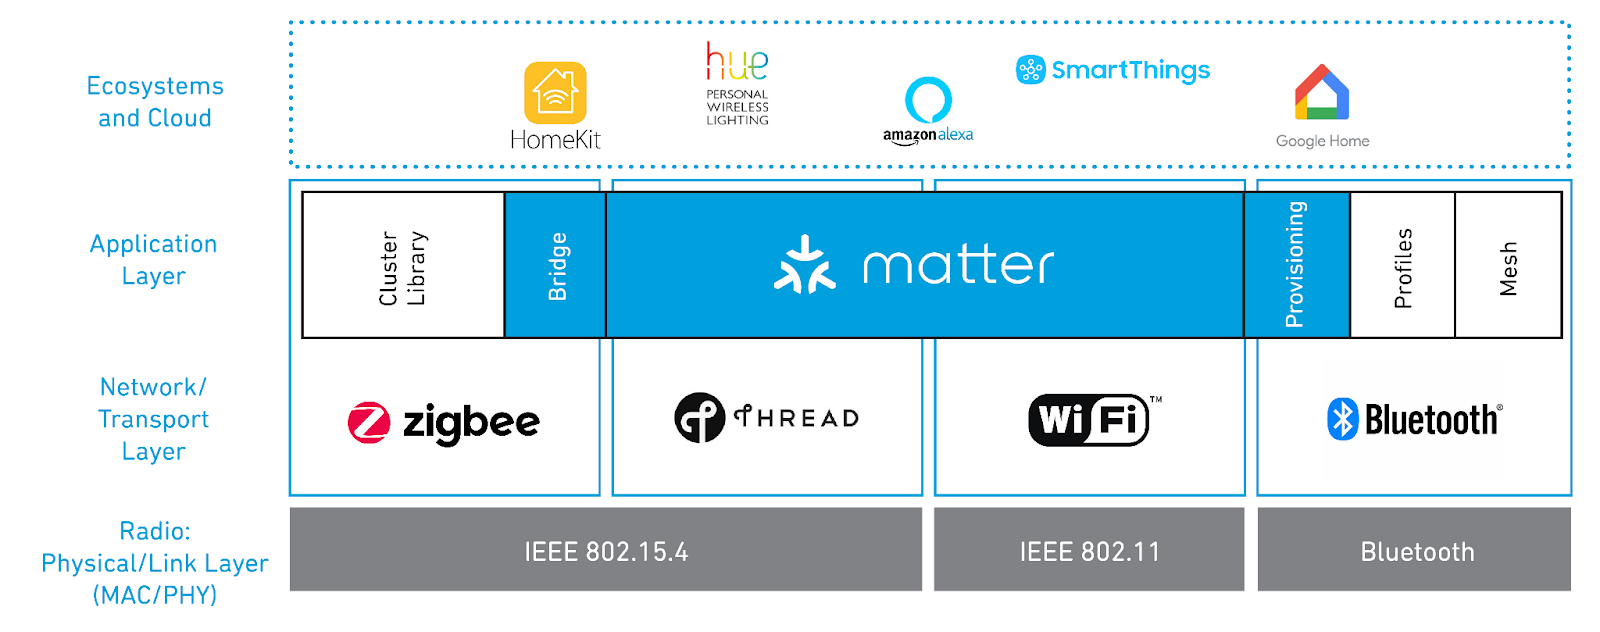
\includegraphics[width=0.9\textwidth]{DescricaoProcesso/Figuras/matter_big_arc.png}
  \caption{Arquitetura do \textit{Matter} como camada de aplicação.}
  \label{fig:matter-layer}
\end{figure}

Como descrito em \cite{matter_spec}, o protocolo Matter garante interoperabilidade entre diferentes dispositivos.

\subsection{Interface de Usuário}

A interface de usuário conecta pessoas e sistema, permitindo controle e monitoramento:

\begin{itemize}
    \item \textbf{Aplicativos Móveis e Web}: Acesso em qualquer lugar, visualização de histórico, criação de cenários e recebimento de notificações.
    \item \textbf{Painéis Físicos}: Telas sensíveis ao toque instaladas nas paredes, facilitando ajustes rápidos.
    \item \textbf{Assistentes Virtuais de Voz}: Google Assistant, Alexa, Siri, oferecendo controle sem a necessidade de interfaces gráficas.
\end{itemize}

Com o \textit{Matter}, a experiência do usuário é aprimorada, pois um único aplicativo ou assistente pode controlar dispositivos de diferentes marcas.

\subsection{Serviços em Nuvem e Análise de Dados}

A nuvem possibilita armazenamento histórico, análise avançada e integração com serviços externos:

\begin{itemize}
    \item \textbf{Análise Preditiva}: Antecipar consumos futuros, otimizar uso de energia.
    \item \textbf{Tarifas Dinâmicas}: Ajustar consumo conforme variação de preços de energia.
    \item \textbf{Manutenção Preditiva}: Identificar falhas iminentes em equipamentos.
\end{itemize}

A nuvem também permite acesso remoto, controle global e integração de APIs de terceiros, ampliando a funcionalidade do sistema.

\subsection{Segurança e Privacidade}

A crescente conectividade na automação residencial traz desafios que vão além de questões técnicas, abrangendo também a proteção de dados e o cumprimento de leis como a Lei Geral de Proteção de Dados (LGPD) no Brasil e o Regulamento Geral sobre a Proteção de Dados (GDPR) na União Europeia. Nesse contexto, é indispensável adotar medidas de segurança cibernética e garantir a privacidade dos moradores, protegendo suas informações pessoais e rotinas. O sistema deve incorporar, desde a fase de projeto, uma abordagem de \textit{Privacy by Design}, assegurando que mecanismos de proteção e conformidade estejam integrados às suas camadas mais básicas.

As principais práticas incluem:

- \textbf{Criptografia}: Todos os dados sensíveis coletados, transmitidos e armazenados devem ser protegidos por criptografia robusta, tornando-os ilegíveis a terceiros não autorizados. Assim, mesmo em caso de interceptação do tráfego de rede, informações pessoais não serão expostas, cumprindo princípios de segurança e confidencialidade exigidos pela LGPD.

- \textbf{Autenticação de Dispositivos}: Garantir que apenas dispositivos autenticados e confiáveis acessem a rede doméstica. Isso envolve a implementação de certificados digitais, chaves criptográficas ou outros métodos de autenticação forte. A restrição de acesso a dispositivos não autorizados previne usos indevidos das informações e atende aos princípios de prevenção e segurança previstos na LGPD.

- \textbf{Atualizações Seguras}: Manter o firmware dos dispositivos atualizado, corrigindo vulnerabilidades e garantindo um nível adequado de segurança contínua. O processo de atualização deve ser autenticado e seguro, impedindo que versões maliciosas sejam instaladas. Essa prática previne incidentes que possam expor dados pessoais e assegura a conformidade com a LGPD, pois reduz o risco de violações de segurança.

A privacidade é igualmente crítica. Dados sobre hábitos e rotinas dos moradores, bem como informações sobre ocupação da residência, uso de dispositivos específicos e preferências pessoais, devem ser armazenados e processados de modo a garantir o respeito à LGPD. Isso significa adotar princípios como minimização da coleta de dados (coletar apenas o indispensável para a finalidade proposta), consentimento informado dos usuários, transparência sobre como e por que os dados são usados e possibilidade de exclusão dos mesmos mediante solicitação. Além disso, todas as práticas de tratamento de dados devem estar documentadas e auditáveis, para comprovação de conformidade quando necessário.

\subsection{Integração com Outros Sistemas}

A automação residencial não funciona isoladamente. Ela pode integrar-se a sistemas de segurança, entretenimento, eletrodomésticos inteligentes e geração distribuída de energia, formando um ecossistema mais rico e funcional. Por exemplo, o sistema pode ajustar o uso de energia com base na produção solar local ou desativar determinados dispositivos ao detectar que a casa está vazia. No entanto, ao integrar múltiplos sistemas e plataformas, a complexidade na gestão dos dados aumenta. Nesse cenário, é fundamental garantir que todos os serviços externos cumpram também as normas de privacidade e segurança, incluindo a LGPD, mantendo assim a coerência e a proteção dos dados em todo o ecossistema.

\subsection{Escalabilidade e Flexibilidade}

A capacidade de crescer e se adaptar às mudanças é vital. Um sistema de automação residencial deve suportar a adição de novos dispositivos, tecnologias e serviços sem exigir reestruturações complexas. O uso de padrões abertos, como o \textit{Matter}, fortalece a escalabilidade e flexibilidade, garantindo que o sistema possa evoluir junto com o usuário e o mercado. Neste contexto, qualquer expansão deve manter o mesmo nível de conformidade com a LGPD, ampliando as práticas de segurança e privacidade para acomodar novos fluxos de dados, dispositivos e funcionalidades sem comprometer a proteção das informações pessoais.

\subsection{Instrumentação do Processo}

A instrumentação do processo envolve a seleção, instalação e configuração de sensores, atuadores e controladores. Esse cuidado na instrumentação não apenas assegura a qualidade dos dados e a efetividade das ações executadas, como também garante que o tratamento das informações coletadas obedeça aos princípios da LGPD e demais normas de proteção de dados. Para isso, alguns cuidados adicionais devem ser tomados:

- \textbf{Seleção de Hardware}: Além de atender às faixas de operação e às especificações técnicas, é importante escolher sensores e atuadores de fabricantes comprometidos com práticas adequadas de segurança e privacidade. O hardware deve permitir a implementação de criptografia, controle de acesso e atualizações seguras. Dispositivos que já seguem padrões abertos e oferecem mecanismos de proteção de dados facilitam a conformidade legal.

- \textbf{Topologia da Rede}: Ao projetar a rede, deve-se garantir cobertura de sinal, minimizar interferências e assegurar redundância em redes \textit{mesh}. Além da confiabilidade técnica, a topologia deve permitir segmentação da rede, isolando dispositivos críticos daqueles com maior risco de vulnerabilidades. Essa separação física ou lógica dificulta acessos não autorizados a dados sensíveis, contribuindo para a privacidade e segurança dos moradores.

- \textbf{Integração Elétrica}: A correta instalação elétrica, observando segurança, aterramento, fusíveis e normas técnicas, assegura não apenas o bom funcionamento dos componentes, mas também evita falhas que possam comprometer a segurança das informações. Curto-circuitos ou picos de tensão inesperados podem afetar módulos de segurança, chaves criptográficas ou até mesmo corromper dados sensíveis.

- \textbf{Provisionamento de Dispositivos}: A configuração inicial dos endereços, chaves de segurança e rotinas de atualização deve ser realizada de forma segura, garantindo que o dispositivo só seja controlado por usuários autorizados. Além disso, políticas de senhas fortes, autenticação de dois fatores e gestão de chaves criptográficas são práticas recomendadas. Essa etapa é essencial para assegurar conformidade com a LGPD, já que uma falha na configuração inicial pode resultar em acesso indevido a dados pessoais, comprometendo a privacidade dos moradores.

Em suma, a instrumentação não é apenas um aspecto técnico; ela é o alicerce para a proteção dos dados, a manutenção da segurança e o respeito à privacidade. Ao combinar boas práticas de engenharia com requisitos legais, o sistema de automação residencial pode operar de forma confiável, eficiente e em total conformidade com a LGPD e outras normas de proteção de dados.

\section{Monitoramento Energético}
\label{sec:monitoramento_energetico}

O monitoramento energético é um elemento central para a compreensão aprofundada do uso de recursos em um ambiente residencial automatizado. Mais do que simplesmente quantificar o consumo de eletricidade, o monitoramento energético permite revelar padrões, prever demandas futuras, identificar ineficiências e propor intervenções corretivas ou preventivas. Ao integrar dados provenientes de diversos sensores — incluindo aqueles dedicados à medição de corrente e tensão em circuitos específicos, bem como às tomadas e equipamentos inteligentes —, o sistema obtém uma visão holística do comportamento energético da residência.

Abaixo, são detalhadas as principais etapas e aspectos relacionados ao monitoramento energético, com especial ênfase na análise de dados, privacidade, conformidade com a LGPD, aplicações práticas e o uso de técnicas de controle estatístico de processo.
\subsection{Coleta e Organização dos Dados}

A primeira etapa do monitoramento energético consiste na coleta sistemática de dados relativos ao consumo de eletricidade em diferentes pontos da residência. Esses dados podem ser obtidos por meio de:

\begin{itemize}
    \item \textbf{Sensores de Consumo em Tempo Real}: Dispositivos que medem corrente e tensão, permitindo o cálculo instantâneo da potência e energia consumidas em circuitos específicos ou em eletrodomésticos individuais.
    \item \textbf{Tomadas e Disjuntores Inteligentes}: Elementos capazes de registrar o uso energético de um aparelho conectado, bem como ligar ou desligar o fornecimento conforme instruções do controlador.
    \item \textbf{Medição Global da Residência}: Sensores posicionados no quadro elétrico principal, fornecendo uma visão macro do consumo, contra a qual se podem comparar dados mais granulares para identificar fontes de ineficiência.
\end{itemize}

A coleta contínua gera um grande volume de dados. Para lidar com isso, é essencial adotar uma infraestrutura de armazenamento e processamento robusta. Uma opção comum é o uso de um \textbf{NAS (Network Attached Storage)}, um dispositivo de armazenamento conectado à rede local que fornece espaço centralizado e seguro para arquivamento dos dados. O NAS permite acesso controlado, backup automático e fácil ampliação da capacidade de armazenamento. Além disso, a utilização de sistemas em nuvem, servidores locais ou híbridos pode complementar o NAS, garantindo resiliência, segurança e acessibilidade dos dados.

Em qualquer cenário, devem-se implementar mecanismos de segurança (criptografia, autenticação forte) e compressão/normalização para facilitar o processamento posterior.

\subsection{Pré-Processamento, Qualidade dos Dados e Controle Estatístico de Processo}

Antes de realizar análises avançadas, os dados coletados precisam passar por etapas de pré-processamento, incluindo:

\begin{itemize}
    \item \textbf{Limpeza de Dados}: Remoção de leituras espúrias, tratamento de valores faltantes e correção de discrepâncias causadas por ruído elétrico ou falhas de comunicação.
    \item \textbf{Agregação e Granularidade}: Ajuste da escala temporal (por exemplo, sumarizar leituras segundo a segundo, minuto a minuto ou hora a hora) e espacial (agrupando dados por cômodo, circuito ou categoria de aparelho).
    \item \textbf{Normalização e Padronização}: Transformação dos dados em escalas comparáveis, permitindo análises consistentes entre diferentes pontos de medição ou períodos.
\end{itemize}

Um conjunto de dados bem pré-processado é mais coerente, confiável e adequado à aplicação de técnicas de análise estatística, aprendizado de máquina e modelagem preditiva.

Nesse contexto, o \textbf{Controle Estatístico de Processo (CEP)} pode ser aplicado ao monitoramento energético como uma ferramenta para acompanhar a variabilidade do consumo ao longo do tempo. Oriundo do domínio da qualidade industrial, o CEP utiliza gráficos de controle e limites estatísticos para distinguir variações normais de anomalias. Aplicado à automação residencial, o CEP permite:

\begin{itemize}
    \item \textbf{Estabelecer Faixas Normais de Operação}: Determinar limites superiores e inferiores para o consumo esperado, considerando padrões históricos e características da residência.
    \item \textbf{Detecção Precoce de Anomalias}: Identificar rapidamente desvios significativos, como um aumento inesperado no consumo de um aparelho, indicando falha ou uso indevido.
    \item \textbf{Monitoramento Contínuo}: Acompanhar a evolução do consumo ao longo do tempo, avaliando se as mudanças implementadas (como troca de um equipamento ou ajuste nas rotinas) resultam em maior eficiência.
\end{itemize}

O CEP atua como um complemento às técnicas de análise mais complexas, ajudando a manter o sistema dentro de parâmetros normais e fornecendo bases para intervenções pontuais.
\subsection{Análise Estatística e Inteligência Artificial}
Com dados limpos e estruturados, bem como limites estatísticos definidos pelo CEP, torna-se possível aplicar uma variedade de técnicas analíticas para extrair valor significativo:

\begin{itemize}
    \item \textbf{Estatística Descritiva}: Cálculo de médias, medianas, desvios-padrão e percentis para caracterizar o perfil de consumo energético ao longo do tempo.
    \item \textbf{Detecção de Anomalias Avançada}: Em conjunto com o CEP, métodos de aprendizado de máquina podem reconhecer padrões não lineares, detectando anomalias sutis que escapariam a métodos estatísticos convencionais.
    \item \textbf{Análise de Correlação e Causalidade}: Estabelecer relações entre o consumo energético e outras variáveis (temperatura, ocupação, eventos externos).
    \item \textbf{Modelagem Preditiva}: Uso de algoritmos de aprendizado supervisionado ou não supervisionado para prever demandas futuras, ajustar parâmetros de controle em tempo real e recomendar intervenções.
    \item \textbf{Clusterização de Perfis de Consumo}: Agrupamento de padrões de uso semelhantes, auxiliando na identificação de zonas energéticas e na otimização personalizada do sistema.
\end{itemize}

A inteligência artificial, combinada ao CEP, amplia as capacidades do sistema, tornando-o mais adaptativo e robusto. Isso resulta em ajustes proativos na operação da residência, reduzindo custos, melhorando o conforto e minimizando impactos ambientais.

\subsection{Privacidade, LGPD e Proteção dos Dados Energéticos}

As informações sobre consumo energético podem revelar hábitos, presença, rotinas e preferências dos moradores. Como tais dados podem ser considerados pessoais ou sensíveis segundo a LGPD, devem ser tratados com o mesmo rigor aplicado a outras informações coletadas:

\begin{itemize}
    \item \textbf{Minimização de Dados}: Coletar apenas o nível de detalhe necessário.  
    \item \textbf{Anonimização e Pseudonimização}: Remover ou mascarar informações identificadoras.
    \item \textbf{Consentimento e Transparência}: Explicar claramente aos moradores como, por que e por quanto tempo os dados serão coletados, analisados e armazenados.
    \item \textbf{Segurança da Informação}: Aplicar criptografia ponta a ponta, autenticação robusta e isolamento de redes.
    \item \textbf{Auditorias e Responsabilização}: Manter registros sobre o tratamento de dados, comprovando conformidade com a LGPD em caso de inspeções.
\end{itemize}

Ao equilibrar análise de dados avançada, CEP e privacidade, o monitoramento energético torna-se não apenas um recurso valioso, mas também uma solução respeitosa aos direitos e expectativas dos usuários.

\subsection{Integração com Outros Sistemas e Evolução Contínua}

O monitoramento energético não existe isoladamente. Ao integrar-se com controladores, sistemas de climatização, iluminação e segurança, bem como com serviços em nuvem e APIs externas, o sistema pode ajustar em tempo real o uso de energia conforme necessidades, demandas e condições externas.

Com a aplicação do CEP, é possível identificar se as integrações e ajustes recomendados estão mantendo o consumo dentro dos limites estatísticos esperados ou se intervenções adicionais são necessárias. Conforme novos dispositivos e tecnologias surgem, a arquitetura flexível e o uso de padrões abertos, como o \textit{Matter}, asseguram que o sistema seja escalável e possa incorporar inovações sem comprometer a segurança, a privacidade ou a qualidade da análise de dados.
\subsection{Benefícios Práticos e Responsabilidade Social}

Quando bem implementado, o monitoramento energético, aliado ao CEP e à análise de dados, traz diversos benefícios:

\begin{itemize}
    \item \textbf{Eficiência e Economia}: Redução de custos com energia elétrica por meio da identificação de desperdícios e ajustes estratégicos.
    \item \textbf{Conforto e Qualidade de Vida}: Ajustes automáticos de parâmetros ambientais conforme preferências e necessidades, sem intervenção manual constante.
    \item \textbf{Sustentabilidade}: Otimização do uso de energia, priorizando fontes renováveis e reduzindo a pegada de carbono.
    \item \textbf{Tomada de Decisão Baseada em Evidências}: Dados claros, validados e dentro de parâmetros estatísticos auxiliares guiam melhorias contínuas e embasadas em fatos.
\end{itemize}

A responsabilidade social emerge ao assegurar que tais benefícios sejam obtidos sem invadir a privacidade ou violar direitos fundamentais. A conformidade com a LGPD, o uso ético da análise de dados e a adoção de CEP garantem que a tecnologia melhore a vida dos moradores, mantendo a confiança e a proteção das informações pessoais.
Em síntese, o monitoramento energético aplicado a um sistema de automação residencial, quando embasado em um arcabouço analítico sólido, conformidade regulatória, uso de CEP e cuidado com a privacidade, transcende a mera coleta de dados. Ele estabelece um processo contínuo de aprendizado, ajuste e otimização que beneficia usuários, meio ambiente e sociedade em geral.  
\bibliography{Monografia}%,library}
\chapter{Metodologia}

Neste capítulo, são detalhadas as etapas metodológicas adotadas no desenvolvimento do sistema inteligente para monitoramento e previsão do consumo de energia residencial. A abordagem foi projetada para atender aos objetivos do projeto, combinando análise técnica, desenvolvimento de soluções e validação experimental. Os procedimentos descritos têm como objetivo garantir a reprodução, escalabilidade e eficácia do sistema proposto, contribuindo para o avanço na área de automação e eficiência energética.

\section{Pesquisa e Análise de Tecnologias Existentes}

A fase inicial do projeto consistiu na identificação e análise das tecnologias disponíveis no mercado para o monitoramento de consumo energético em residências. Esta etapa foi guiada por uma revisão bibliográfica abrangente e um estudo comparativo das soluções existentes, considerando os seguintes critérios:

\begin{itemize}
    \item \textbf{Compatibilidade com infraestruturas residenciais convencionais}: Tecnologias que não exigem modificações estruturais significativas, como sensores de fácil instalação e dispositivos autônomos.
    \item \textbf{Eficiência técnica}: Precisão na coleta de dados, robustez e confiabilidade das medições.
    \item \textbf{Interoperabilidade}: Capacidade de integração com diferentes sistemas e protocolos, como Wi-Fi, Zigbee e Bluetooth Low Energy.
    \item \textbf{Custo-benefício}: Viabilidade econômica para implementação em larga escala.
\end{itemize}

A análise resultou na seleção de componentes que atendem aos requisitos do projeto. Foi escolhida a linha de tomadas \textit{Tuya Smart Wi-Fi}, cuja modularidade permite fácil instalação em diversos locais, utilizando a metodologia \textit{plug and play}. Estas tomadas oferecem integração com a plataforma \textit{Tuya Cloud} e suas APIs, garantindo flexibilidade e escalabilidade.

\section{Desenvolvimento do Protótipo}

Com base nas tecnologias identificadas, foi desenvolvido um protótipo funcional que integra hardware e software para monitoramento e previsão de consumo energético. O desenvolvimento seguiu as seguintes etapas:

\subsection{Seleção e Configuração de Sensores}

As tomadas \textit{Tuya Smart Wi-Fi} foram configuradas para monitorar o consumo energético em tempo real. Estes dispositivos enviam os dados para a plataforma \textit{Tuya Cloud}, de onde são acessados por meio de APIs.

\subsection{Desenvolvimento do Sistema de Controle}

O sistema de controle foi desenvolvido utilizando as APIs fornecidas pela \textit{Tuya Cloud}, permitindo a comunicação entre as tomadas e o sistema central. O controlador é responsável por:

\begin{itemize}
    \item Receber e processar os dados coletados pelas tomadas.
    \item Aplicar algoritmos de análise e previsão de consumo.
    \item Integrar os dados a uma interface de visualização desenvolvida especificamente para o projeto.
\end{itemize}

\subsection{Desenvolvimento da Interface de Visualização}

A interface de monitoramento foi desenvolvida pelo autor do trabalho utilizando linguagens de programação voltadas para desenvolvimento web e visualização de dados. Esta interface exibe de forma intuitiva os padrões de consumo energético, permitindo que os usuários identifiquem desperdícios e ajustem seu comportamento para otimizar o uso de energia.

\section{Implementação de Algoritmos de Processamento e Previsão}

Para o tratamento dos dados coletados, foram desenvolvidos e implementados algoritmos específicos, detalhados a seguir:

\subsection{Pré-processamento dos Dados}

Os dados brutos coletados pelas tomadas passaram por etapas de limpeza e normalização, eliminando leituras espúrias e garantindo consistência nos resultados.

\subsection{Análise Estatística e Controle Estatístico de Processos (CEP)}

O CEP foi utilizado para identificar variações significativas no consumo energético, estabelecendo limites de controle e detectando anomalias. Esta abordagem foi complementada por métodos estatísticos descritivos para caracterizar os padrões de consumo.

\subsection{Previsão de Consumo com Inteligência Artificial}

Modelos de aprendizado de máquina foram treinados utilizando dados históricos para prever demandas futuras de energia. Técnicas como regressão linear e redes neurais foram aplicadas, visando maior precisão e adaptabilidade.

\section{Validação em Ambiente Real}

O protótipo foi testado em um ambiente residencial que não possuía infraestrutura prévia de automação. A validação envolveu:

\begin{itemize}
    \item \textbf{Avaliação de desempenho}: Testes para verificar a precisão das tomadas \textit{Tuya Smart Wi-Fi} e a eficiência dos algoritmos.
    \item \textbf{Usabilidade}: Análise da interface para garantir que usuários finais pudessem interpretar os dados facilmente.
    \item \textbf{Robustez}: Monitoramento contínuo em condições reais, avaliando a resiliência do sistema a falhas.
\end{itemize}

Os resultados dos testes foram documentados e utilizados para refinar o sistema, corrigindo inconsistências e melhorando sua eficiência.

\section{Viabilidade de Implementação em Larga Escala}

A análise de viabilidade considerou aspectos técnicos, econômicos e sociais, como:

\begin{itemize}
    \item \textbf{Custos de produção}: Avaliação dos investimentos necessários para replicação do sistema.
    \item \textbf{Benefícios econômicos}: Potencial de redução de custos para os usuários com base na diminuição do desperdício energético.
    \item \textbf{Impactos ambientais}: Contribuição para a sustentabilidade por meio do uso eficiente de energia.
    \item \textbf{Estratégias de adoção}: Identificação de barreiras e propostas para ampliar o alcance do sistema, como parcerias com fabricantes de dispositivos inteligentes.
\end{itemize}

\section{Resumo do Capítulo}

Este capítulo detalhou as etapas metodológicas seguidas no desenvolvimento do sistema inteligente para monitoramento e previsão de consumo de energia residencial. As etapas compreenderam a análise de tecnologias, desenvolvimento do protótipo utilizando as tomadas \textit{Tuya Smart Wi-Fi}, implementação de algoritmos avançados, validação experimental e estudo de viabilidade em larga escala. A abordagem proposta combina rigor técnico e aplicabilidade prática, destacando-se como uma solução promissora para o setor de automação residencial.
\chapter{Resultados}

Para a execução do projeto, algumas etapas de desenvolvimento tiveram de ser seguidas: familiarização com o sistema, estudo dos módulos envolvidos, leitura dos requisitos, elaboração de documento descrevendo todo o processo de implementação e relacionamento com os diversos módulos, implementação e testes.


\section{Atividades do Projeto}
\label{metodo3}

\section {Requisitos do Sistema}
\label{req}


\section{Desenvolvimeto e Implementação}

A Tabela \ref{tab:tabela} apresenta as atividades executadas.

\begin{table}
\centering
%Note os alinhamentos diferentes em cada coluna
\begin{tabular}{|c|r|l|}\hline
		Atividade 1 & aa  & ab  \\ 
					 & a & b \\ \hline
		Ativ. 2  & aa & ab \\			
					 &  a & b \\ \hline
		\end{tabular}
	\caption{Exemplo de tabela - Coloque toda informação sobre a tabela aqui}
	\label{tab:tabela}
\end{table}

\section{Testes}

\section{Análise dos Resultados}

Apresente os resultados sem adulterações e faça análises objetivas. Pense na melhor maneira de apresentar os resultados graficamente. Se os gráficos são difíceis de interpretar, talvez tabelas sejam uma forma melhor de apresentar resultados. Não apresente dados (gráficos e tabelas) se não há uma conclusão interessante a ser tirada. Lembre-se de ser conciso.

\emph{Não se esqueça das unidades!} Pense que \emph{a priori} todo número deve ter uma unidade. Não escreva as unidades em itálico (no ambiente matemático) e tome cuidado para diferenciar maiúsculas e minúsculas. Um exemplo é escrever $22$ [kN] e não $22 KN$ (Kelvin vezes Newton!).

Ao apresentar resultados experimentais, tome o cuidado para também apresentar o cálculo das incertezas sempre que forem significativas. Ao fazer conclusões, sempre considere se o tamanho da sua amostra é grande o suficiente do ponto de vista estatístico. Lembre que a média empírica $\hat{\mu}_X$ de $N$ observações independentes da variável $X_i$ possui variância
\[
\hat{\sigma}_{\mu}^2 = \frac{1}{N(N-1)} \sum_{i=1}^N (X_i-\hat{\mu}_X)^2
\enspace,
\]
onde se assume que as variáveis $X_i$ possuem uma mesma ditribuição e que essa distribuição possui segundo momento finito.


\section{Resumo do Capítulo}
\label{sec:resumoo4}
Tente não terminar de forma abrupta. Se for escrever algo aqui, não seja genérico!

\section{Formato, expressões matemáticas e o \LaTeX}

\subsection{O \LaTeX}

O {\LaTeX}  é o método preferencial de preparação de documentos para textos técnicos nas ciências exatas. O {\LaTeX} permite não só lidar com equações de uma forma mais prática que em editores de texto, mas também facilita a formatação de documentos e tem um desempenho marcadamente superior a editores de texto na preparação de documentos longos como monografias. 

Documentos em {\LaTeX} são escritos em um ou mais arquivos de texto com extensão .tex. Após a escrita, o .tex é \emph{compilado} para gerar arquivos nos formatos .pdf, .dvi ou .ps. Hoje há duas distribuições padrão para o \LaTeX. Sistemas Windows usam o {Mik\TeX} e sistemas Unix usam o \TeX Live. Além das distribuições, muitos usuários utilizam \emph{front-ends} que facilitam a edição do texto, a compilação e a instalação de pacotes. 

Os pacotes necessários para compilar o presente documento devem ser encontrados numa instalação completa dessas distribuições. Se tiver dificuldades com os pacotes, você pode instalá-los manualmente ou tentar alterar o código para usar versões antigas dos mesmos.

A compilação pode ser feita pelos comandos \textsf{latex} ou \textsf{pdflatex}, invocados pela linha de comando ou pelo \emph{front-end}. Note que será necessário empregar o comando \textbf{mais de uma vez} para que as referências cruzadas saiam corretas.

Como discutido na Seção \ref{sec:revisão}, uma ferramenta útil para gerenciar as citações em {\LaTeX} é o Bib\TeX. Para gerar uma lista bibliográfica a partir do arquivo .bib, este arquivo deve ser indicado no arquivo .tex. Em seguida devem-se executar os comandos \textsf{pdflatex}, \textsf{bibtex} e \textsf{pdflatex} novamente sempre usando o .tex como argumento. Note que os comandos são executados nesta ordem e de forma repetida para que as referências cruzadas sejam geradas corretamente.

Nesta seção você deve encontrar exemplos dos comandos mais usados em \LaTeX. Outros exemplos e manuais podem ser encontrados na internet com facilidade.

\subsection{Expressões Matemáticas}

Ao escrever expressões matemáticas, defina todas as variáveis antes de usá-las ou imediatamente depois da expressão. Deixar de fazê-lo torna seu texto \textbf{ilegível}. Segue um exemplo.

Seja o par $(a_1,a_2)\in \mathbb{R}^2$. Para $s\in\mathbb{C}$, definimos a função $f(s)$ como
\[%cria equações sem numeração
f(s)\triangleq \frac{a_1 s+a_2}{s^2+2\zeta\omega_n s+\omega_n^2}
\enspace,
\]
onde os escalares $\zeta,\omega_n>0$ são constantes.

Note que não foi necessário atribuir valores às variáveis neste momento. Repare também como devemos \textbf{usar pontuação} (vírgula) nas equações, tratando-as como parte da frase. Usamos o símbolo $\triangleq$ ou $:=$ para deixar explícito que se trata de uma definição. Ser claro nesse aspecto facilita o entendimento do leitor.

A equação acima não foi numerada porque não será citada no texto. Vejamos um exemplo com numeração.

A função $f(\cdot)$ possui um zero em $-a_2/a_1$ (ou $-\frac{a_2}{a_1}$) e, para $\zeta<1$, possui polos complexos $p_{1,2}$ dados por
\begin{equation}
\label{eq:polos}
p_{1,2}=\omega_n \left(-\zeta\pm j\sqrt{1-\zeta^2}\right)
\enspace.
\end{equation}
Agora podemos citar os polos dados pela Equação (\ref{eq:polos}) (aqui adotamos a convenção de citar sempre com o número entre parênteses precedido da palavra Equação). Note como usamos um comando especial na Equação \ref{eq:polos} para garantir o ajuste automático do tamanho dos parênteses.

Vejamos agora como criar equações alinhadas. Considere o sistema dinâmico dado pelas equações diferenciais:

\begin{align}
\dot{x}_1 & = \cos(x_2)\cdot\ln(1/x_1)+\tan(u) \label{eq:x1dot} \\
\dot{x}_2 & = e^{-x_1-x_2} \nonumber \\
& y  = \min\{x_1,x_2\}  \label{eq:saida}
\enspace,
\end{align}
onde $x(t)=[x_1(t) ~ x_2(t)]'$, $t>0$, é a variável de estado do sistema, $u(t)$ é o sinal de entrada e $y(t)$ é o sinal de saída do sistema. Note no .tex que o caracter de tabulação \textsf{\&} foi usado para indicar o ponto de alinhamento horizontal das equações. Além disso, para ilustrar o uso do \LaTeX, retiramos a numeração da segunda equação e citamos as equações separadamente.

Nas Equações (\ref{eq:x1dot}) e (\ref{eq:saida}), aparecem operadores como $\min$, $\ln$, $\cos$ e $\tan$. A convenção aqui é que \textbf{variáveis devem ser escritas em itálico e operadores não}. Por essa razão todas as expressões matemáticas devem ser escritas no ambiente matemático (entre cifrão) mesmo quando for possível usar texto comum. Isso garante a consistência das fontes utilizadas (nem sempre a fonte do ambiente matemático é a mesma fonte do texto). 

Para escrever matrizes, podemos fazer por exemplo:
\[
\sum_{n=0}^{\infty}z^{-n}\left[\begin{array}{cc}
\lambda & 1 \\
0 & \lambda
\end{array}\right]^n=
\left[\begin{array}{cc}
\frac{z}{z-\lambda} & \frac{z}{(z-\lambda)^2} \\
0 & \frac{z}{z-\lambda}
\end{array}\right]
,~\forall \lambda<|z|
\enspace.
\]

Para escrever uma expressão com múltiplos casos, podemos fazer, para um inteiro $N$ positivo,
\[
g[n]=
\left\{
\begin{array}{ll}
0,& \mbox{se }~ n\leq 0 \\
n,& \mbox{se }~ n=1,2,\ldots,N-1 \\
N,& \mbox{se }~ n\mod N = 0 \\
0,& \mbox{caso contrário}\enspace.
\end{array}
\right.
\]

\textbf{Nunca reaproveite símbolos} matemáticos, isto é, nunca use o mesmo símbolo para designar variáveis diferentes.

Para um exemplo com múltiplas linhas de expressão matemática: tem-se que, para $a\neq 0$,

\begin{equation}
\begin{split}
ax^2+bx+c &= 0 \\
& \Rightarrow a(x^2+bx/a+c/a) =0 \Rightarrow a((x+b/(2a))^2+c/a-b^2/(4a^2))=0  \\
& \Rightarrow (x+b/(2a))^2=(b^2-4ac)/(4a^2) \\
& \Rightarrow (x+b/(2a))=\pm\sqrt{b^2-4ac}/(2a) \\
& \Rightarrow x=\frac{-b\pm\sqrt{b^2-4ac}}{2a}
\enspace.
\end{split}
\end{equation}

Note a argumentação lógica aqui. Não estamos dizendo que o valor de $x$ é dado pela última linha. Estamos dizendo que a hipótese da primeira linha juntamente com a hipótese $a\neq 0$ implicam os referidos valores de $x$. \textbf{Um erro comum dos alunos ao escrever é não distinguir a veracidade das implicações com a veracidade das hipóteses}.

\clearpage
\chapter{Conclusões}

Novamente, este será um dos trechos que o leitor experiente lerá antes de decidir se vale a pena ler o texto integral. Seja convincente.

\section{Considerações Finais}

Reitere o que de mais importante foi feito, qual era o objetivo inicial e qual o resultado obtido. Se houve requisitos ou especificações de projeto, discuta se foram atingidos. Se os resultados não foram conclusivos ou contrariam o que se esperava, seja honesto e diga-o explicitamente. Busque explicar os insucessos com argumentos sólidos e plausíveis. 

\section{Propostas de Continuidade}

Se houve questões ainda não respondidas ou resultados insatisfatórios, aponte direções de continuação.

\clearpage


\addcontentsline{toc}{chapter}{Referências Bibliográficas}
\renewcommand{\bibname}{Referências Bibliográficas}

%\bibliographystyle{abntex2-alf} %para norma ABNT no sistema autor-data
\bibliographystyle{abntex2-num}
\begin{small}

%% Monografia para Projeto de Fim de Curso - Exemplo no LaTeX
%-----------------------------------------------------------


%---------------Inicialização de pacotes--------------------

\documentclass[12pt,a4paper,notitlepage,twoside]{book}


\usepackage{graphicx}
\usepackage[utf8]{inputenc}
%\usepackage[latin1]{inputenc} %%pode ser necessário trocar a codificação em sistemas Windows
\usepackage[brazil]{babel}		%%pode ser necessário trocar o pacote de línguas em algumas distribuições LateX
%\usepackage[portuguese]{babel}
\usepackage[T1]{fontenc}
\usepackage{amsmath,amssymb}
\usepackage{amsthm,amsfonts}
\usepackage{color}
\usepackage[colorlinks]{hyperref}
\usepackage{abntex2abrev}
%\usepackage[alf]{abntex2cite} %se você quiser seguir as normas ABNT no sistema autor-data
%\usepackage[num]{abntex2cite} %se você quiser seguir as normas ABNT no sistema numérico
\usepackage{setspace}
\usepackage[toc,page]{appendix}

%Definindo fonte Times (Use os pacotes obsoletos se não conseguir instalar os atualizados)
%\usepackage{times}     %Pacote de fontes obsoleto, apenas texto
%usepackage{mathptmx}  %Pacote de fontes obsoleto, texto e símbolos matemáticos
%\usepackage{newtxtext,newtxmath}  %Pacotes de fontes mais recentes

\usepackage[a4paper,top=30mm,bottom=30mm,inner=30mm,outer=25mm,headheight=7mm,headsep=6mm,footskip=7mm]{geometry}
\usepackage{enumerate}

\makeindex

%\singlespacing   %%espaçamento simples
%\onehalfspacing
%\setstretch{1.03} %%um pouco melhor que espaçamento simples
\linespread{1.25} %corresponde ao espaçamento 1.5 do MS Word

%---------------Início do documento-------------------------

\begin{document}

\begin{titlepage}
\begin{center}
{\large Universidade Federal de Minas Gerais\\
Escola de Engenharia \\
Curso de Graduação em Engenharia de Controle e Automação\\}

\vspace{6cm}
{\bf\Large Monitoramento e previsão do consumo de energia residencial baseado em Sistemas
Inteligentes\vspace{0.2cm}}

\vspace{4cm}

%\hspace{0.3\textwidth} \parbox{0.65\textwidth}
{\large Igor Cleto Silva de Araújo}
\vspace{2cm}  
   
\vspace{2cm}          
%\hspace{0.3\textwidth} 
{\large Orientadora: Prof Carmela Maria Polito Braga}\\

\vfill
%\hspace{0.3\textwidth} 
{\large Belo Horizonte, Outubro de 2024 }
\end{center}

\end{titlepage}

\newpage
\clearpage
\thispagestyle{empty}


\begin{titlepage}

\centering
\textbf{Monografia}\\
\vspace{2cm}
\centering
\textbf{Monitoramento e previsão do consumo de energia residencial baseado em Sistemas
Inteligentes}\\
\vspace{5cm} 

\parbox{1.0\textwidth} 
{\large 
Monografia submetida à banca examinadora
designada pelo Colegiado Didático do Curso de
Graduação em Engenharia de Controle e
Automação da Universidade Federal de Minas
Gerais, como parte dos requisitos para aprovação na
atividade Projeto Final de Curso II.}

\vspace{7cm} 
\centering
Belo Horizonte, Outubro de 2024

\end{titlepage}


\pagenumbering{roman}
\addcontentsline{toc}{chapter}{Resumo}

\begin{center}
\huge{{\bf Resumo}}
\vspace{2cm}
\end{center}

No Resumo, em uma única página, em no máximo dois parágrafos, você explicita os seguintes itens: objetivos do projeto e descrição sucinta do local onde ele foi desenvolvido; metodologia utilizada; e resultados alcançados. Leitores experientes decidem se prosseguirão para a leitura do texto completo após lerem o resumo, a conclusão e a introdução. Por isso nestes lugares você deve colocar um esforço maior de convencimento. Além disso, a linguagem utilizada deve ser acessível a leitores com pouca familiaridade com a área, limitando-se o uso de jargões.
 
\begin{sloppypar}
Este novo parágrafo serve para mostrar que ao pular uma ou mais linhas no texto do arquivo .tex, o \TeX\ entende que você está iniciando outro parágrafo. O comando \textsf{sloppypar} força o texto a não ultrapassar as margens. Só deve ser usado se este problema ocorrer.
\end{sloppypar}

 
\clearpage
\thispagestyle{empty}
\cleardoublepage


\addcontentsline{toc}{chapter}{Abstract}

\begin{center}
\huge{{\bf Abstract}}
\vspace{2cm}
\end{center}

This project aims to develop an intelligent system for monitoring and forecasting energy consumption in homes that were not originally designed for home automation. Specifically, it seeks to research and analyze existing technologies that allow energy monitoring without requiring prior infrastructure, and to explore solutions suitable for conventional residences. The project will involve the development of a prototype for an easily installable and user-friendly monitoring system, as well as the implementation of data processing algorithms and consumption forecasting using artificial intelligence techniques. An intuitive software platform will be created for users to visualize and analyze the data, and the system will be tested and validated in a real-world environment to ensure its efficiency and usability. To promote the feasibility of large-scale implementation, the project will include cost analysis and strategies for adoption. Finally, the results will be documented and disseminated, emphasizing the contributions to Control and Automation Engineering and the social and environmental benefits provided by the developed system. 

\clearpage
\thispagestyle{empty}
\cleardoublepage


\addcontentsline{toc}{chapter}{Agradecimentos}

\begin{center}
\huge{{\bf Agradecimentos}}
\vspace{4cm}
\end{center}

Gostaria de expressar minha profunda gratidão a Deus, pela saúde física e mental que me permitiu a realização dos meus sonhos e objetivos. Aos meus pais, meu sincero agradecimento pelo suporte incondicional aos meus estudos desde a minha infância, sempre acreditando em meu potencial e me incentivando a seguir em frente. Agradeço também aos meus professores e gestores, que, com seu apoio e ensinamentos, tanto dentro quanto fora da sala de aula, contribuíram para a minha formação acadêmica e pessoal. Não poderia deixar de agradecer, de maneira especial, à minha orientadora, Profª. Carmela Maria Polito Braga, pela dedicação, paciência e orientação ao longo deste um ano de desenvolvimento deste trabalho. Sua contribuição foi fundamental para a realização deste projeto. A todos, meu muito obrigado.
 
\clearpage
\thispagestyle{empty}
\cleardoublepage
\tableofcontents
%\markboth{Conteúdo}{Conteúdo}

\clearpage
%\thispagestyle{empty}
%\cleardoublepage

% Normalmente, este arquivo só contém isto.
\listoffigures
\addcontentsline{toc}{chapter}{Lista de Figuras}
%\markboth{Lista de Figuras}{Lista de Figuras}

\clearpage
%\thispagestyle{empty}
%\cleardoublepage

% Normalmente, este arquivo só contém isto.
\listoftables
\addcontentsline{toc}{chapter}{Lista de Tabelas}
%\markboth{Lista de Tabelas}{Lista de Tabelas}

\clearpage
%\thispagestyle{empty}
%\cleardoublepage

% Normalmente, este arquivo só contém isto.

\pagenumbering{arabic}
\setcounter{page}{1}
\chapter{Introdução}
\label{chap:intro} %este label será usado para referenciar este capítulo

% As primeiras frases têm a missão de prender a atenção do leitor e por isso são as mais importantes do texto. Diga o quanto antes o que você fez e quais são os resultados alcançados. Ao terminar de ler a introdução o leitor tomará uma nova decisão de se vale a pena ou não continuar lendo o texto. Capte a atenção do leitor bem aqui.

% A comunicação escrita é considerada umas das cinco habilidades mais importantes por profissionais de engenharia e um engenheiro passa em média mais de $25$\% do seu tempo escrevendo \cite{eggert2002response,spretnak1982survey}. Uma quantidade similar de tempo é gasta na escrita de correspondência e de relatórios técnicos \cite{cunningham2012perceptions}. Dessa forma, encare a escrita do seu projeto como um treinamento nessa importante habilidade.

% Neste texto você encontrará não apenas uma estrutura para escrever seu trabalho em \LaTeX, mas também um pequeno manual de boas práticas na escrita técnica. Leia com atenção e coloque as sugestões em prática à medida que preenche o texto com o conteúdo do seu próprio projeto. Também será apresentado um número de vícios de escrita comumente encontrados nas monografias de alunos. 

% A seguir está a estrutura de organização sugerida pelo colegiado do curso. Note que ela não é necessariamente a melhor para contar a história do seu projeto. Você pode por exemplo preferir usar títulos mais pertinentes ao seu contexto. Contudo, o seu texto deve conter cada um dos pontos a seguir.

\section{Motivação e Justificativa}
\label{sec:motivacao}

A crescente demanda por energia elétrica, aliada à necessidade de uso eficiente dos recursos energéticos, torna imperativo o desenvolvimento de soluções inovadoras que permitam aos consumidores monitorar e gerenciar seu consumo de forma eficaz e em tempo real. No contexto residencial, muitas vezes os usuários não têm acesso a informações detalhadas sobre o consumo energético em suas casas, o que dificulta a identificação de desperdícios e a implementação de medidas para a redução do consumo. O cenário se agrava devido à falta de sistemas acessíveis e de fácil implementação para o monitoramento eficiente, o que resulta em uma grande dificuldade para os consumidores em adotar práticas mais sustentáveis e econômicas no seu cotidiano. 

Além disso, a automação residencial enfrenta desafios consideráveis relacionados à integração de dispositivos e sensores de diferentes fabricantes. A grande diversidade de tecnologias, protocolos de comunicação e padrões de mercado, somada à ausência de uma padronização efetiva entre os diferentes fabricantes, cria um ambiente no qual os dispositivos muitas vezes não se comunicam de maneira eficiente, impedindo a criação de sistemas unificados de monitoramento e controle. Esse cenário limita os benefícios da automação, como a otimização do consumo de energia e a melhoria da qualidade de vida dos moradores, além de dificultar o acesso a tecnologias que poderiam proporcionar um ambiente mais confortável, seguro e sustentável.

Adicionalmente, muitas residências não foram originalmente projetadas com infraestrutura para automação, o que torna a adaptação desses ambientes ao uso de tecnologias de monitoramento e controle mais complexa e dispendiosa. A implementação de soluções de automação, frequentemente, exige modificações estruturais significativas, que podem tornar o processo oneroso e inviável para uma grande parcela da população. Isso, por sua vez, desencoraja muitos proprietários a adotarem essas tecnologias, deixando uma significativa quantidade de residências sem os benefícios em termos de eficiência energética, conforto e segurança que poderiam ser proporcionados por sistemas de automação. Assim, a falta de alternativas acessíveis e de fácil implementação para o monitoramento e gestão do consumo energético representa uma grande oportunidade de desenvolvimento de soluções que possam superar essas barreiras técnicas e financeiras e beneficiar uma ampla gama de usuários.

\section{Objetivos do Projeto}
\label{sec:objetivos}

Tendo em vista o exposto acima, este projeto tem por objetivos:

\begin{enumerate}[a)]
\item Realizar uma pesquisa e análise de tecnologias existentes que permitam o monitoramento energético sem a necessidade de infraestrutura prévia;
\item Explorar soluções adequadas para residências convencionais, que não foram originalmente projetadas para automação residencial;
\item Desenvolver um protótipo de sistema de monitoramento de fácil instalação e uso;
\item Implementar algoritmos de processamento de dados e previsão de consumo utilizando técnicas de inteligência artificial;
\item Criar uma plataforma de software intuitiva para visualização e análise dos dados pelos usuários;
\item Testar e validar o sistema em ambiente real, garantindo sua eficiência e usabilidade;
\item Promover a viabilidade de implementação em larga escala por meio da análise de custos e estratégias de adoção;
\item Documentar e divulgar os resultados obtidos, destacando as contribuições para a Engenharia de Controle e Automação e os benefícios sociais e ambientais proporcionados pelo sistema desenvolvido.
\end{enumerate}

\section{Local de Realização}
\label{sec:empresa}

O local de realização deste projeto é a residência do próprio desenvolvedor, onde os testes dos equipamentos e a simulação das necessidades reais de automação residencial estão sendo realizados. A escolha deste ambiente se justifica pela possibilidade de realizar uma avaliação prática e realista das soluções de monitoramento e previsão de consumo energético, simulando as condições do dia a dia em uma residência convencional. A residência não foi originalmente projetada com infraestrutura para automação, o que representa um desafio adicional, mas também um aspecto relevante para a validação do sistema, pois permite testar a adaptação de tecnologias em um ambiente que não conta com recursos avançados de automação.

Neste contexto, o projeto visa avaliar a viabilidade de implementação de soluções de monitoramento energético em ambientes residenciais que, assim como muitas casas, não foram concebidos para suportar sistemas automatizados. Dessa forma, o projeto busca não apenas desenvolver uma solução eficiente, mas também uma que seja de fácil adaptação e acessível para a grande maioria dos consumidores. O vínculo com o local de testes é direto, pois, além de ser o ambiente de realização das simulações, a residência do desenvolvedor também serve como um campo de experimentação e validação para os resultados do sistema proposto.

\section{Estrutura da Monografia}
\label{sec:organizacao}

O trabalho está dividido em quatro capítulos. Este capítulo apresentou uma introdução ao projeto descrito nesta monografia, incluindo o objetivo de desenvolvimento de um sistema inteligente para monitoramento e previsão de consumo de energia em residências, além de descrever o local de realização dos testes, que ocorre na residência do próprio desenvolvedor. O Capítulo 2 descreve os princípios básicos de um sistema de automação residencial e monitoramento energético, abordando todos os conceitos necessários para um melhor entendimento do projeto. O Capítulo 3 explora a metodologia de desenvolvimento, incluindo a análise das tecnologias existentes, a criação do protótipo e a implementação dos algoritmos de processamento de dados e previsão de consumo. No Capítulo 4, apresenta-se a conclusão da monografia, com um resumo dos resultados alcançados e algumas sugestões e dificuldades encontradas durante a realização do projeto.

\clearpage
\chapter[Princípios de Automação Residencial]{Princípios básicos de um sistema
de automação residencial e monitoramento energético}
\label{chap:principios}
%Note que, como o nome do capítulo é muito longo, fornecemos um nome abreviado para uso no cabeçalho

Este capítulo apresenta uma visão abrangente dos princípios fundamentais na concepção, implementação e operação de um sistema inteligente de automação residencial orientado ao monitoramento e previsão do consumo energético. O contexto abordado parte da realidade de residências convencionais, isto é, aquelas que não dispõem de infraestrutura prévia de automação, exigindo assim soluções flexíveis, escaláveis e capazes de integrar múltiplos dispositivos e tecnologias. Nosso enfoque não se limita ao simples acionamento de equipamentos, mas abrange a coleta e análise detalhada de dados, permitindo uma gestão mais eficiente dos recursos, redução de custos, melhoria do conforto e incremento da sustentabilidade ambiental.

Iniciamos com um exame minucioso da arquitetura típica de um sistema de automação residencial, descrevendo os principais componentes: sensores (ambientais, de presença, de consumo energético), atuadores (termostatos, dimmers, motores para cortinas, entre outros), controladores (centralizados e distribuídos), protocolos de comunicação (Wi-Fi, Zigbee, Z-Wave, BLE, Thread e \textit{Matter}) e interfaces de usuário (aplicativos, painéis físicos, assistentes de voz). Destacamos, em especial, o \textit{Matter}, um protocolo emergente que unifica e facilita a interoperabilidade entre dispositivos de diferentes fabricantes, garantindo flexibilidade, segurança e escalabilidade ao ecossistema doméstico conectado.

Em seguida, detalhamos o processo de instrumentação do sistema, abordando a seleção criteriosa de hardware, a integração de sensores e atuadores, bem como a definição da topologia da rede. Esse cuidado assegura a qualidade dos dados coletados, a robustez do controle e a adequação às normas legais. A segurança da informação e a privacidade são tratadas de forma transversal, observando-se os princípios da Lei Geral de Proteção de Dados (LGPD) e adotando medidas como criptografia, autenticação de dispositivos, minimização de dados e consentimento informado dos usuários.

Outro ponto central é o monitoramento energético. Não se trata apenas de registrar o consumo, mas de transformar dados brutos em conhecimento. São exploradas técnicas de pré-processamento, análise estatística, aprendizado de máquina e Controle Estatístico de Processo (CEP) para detectar anomalias, identificar padrões de consumo, antecipar demandas e propor intervenções que otimizem o uso de energia. Essas abordagens analíticas embasam decisões proativas, possibilitando desde ajustes automáticos de cargas elétricas até a recomendação de substituição de equipamentos ineficientes, o que resulta em benefícios econômicos, maior conforto e redução do impacto ambiental.

Ao compreender as soluções existentes, suas limitações e potenciais, este capítulo fornece uma base sólida para os desenvolvimentos subsequentes, orientando tanto a implementação prática do protótipo quanto a evolução do sistema no sentido de maior inteligência, integração e respeito à privacidade e às leis vigentes.

\section{Arquitetura de um Sistema de Automação Residencial}

A arquitetura de um sistema de automação residencial é composta por diversos elementos que trabalham em conjunto para oferecer controle, monitoramento e otimização de aspectos como eficiência energética, segurança, conforto e conveniência. Ela não consiste apenas em dispositivos isolados, mas em um ecossistema integrado capaz de entender as condições do ambiente, agir de forma proativa e se adaptar às preferências dos moradores.

A seguir, detalhamos os principais elementos dessa arquitetura, estabelecendo as bases para compreender as complexidades e potencialidades de tais sistemas.

\subsection{Sensores}

Os sensores representam a interface entre o mundo físico e o digital. Eles coletam dados sobre o ambiente e o estado dos dispositivos, fornecendo informações essenciais para que o sistema possa tomar decisões informadas. Podem monitorar temperatura, umidade, luminosidade, qualidade do ar, presença de pessoas e consumo de energia, entre outros parâmetros. Alguns exemplos:

\begin{itemize}
    \item \textbf{Sensores de movimento e presença}: Utilizam tecnologias como infravermelho passivo (PIR), ultrassom ou micro-ondas. Além de acionar luzes ou alarmes, podem colaborar na climatização, ajustando a temperatura apenas em ambientes ocupados.
    \item \textbf{Sensores ambientais (temperatura, umidade, qualidade do ar)}: Auxiliam no controle de sistemas de HVAC (Aquecimento, Ventilação e Ar Condicionado), garantindo conforto térmico e qualidade do ar interno.
    \item \textbf{Sensores de luminosidade}: Ajustam iluminação artificial conforme a luz natural, otimizando o uso de energia e melhorando o bem-estar.
    \item \textbf{Sensores de consumo energético}: Medem o consumo de dispositivos específicos ou circuitos, fornecendo dados granulares para análise, detecção de aparelhos ineficientes e implementação de estratégias de economia de energia.
\end{itemize}

A seleção e instalação adequadas dos sensores são fundamentais, influenciando a qualidade dos dados coletados e a efetividade das estratégias de controle.

\subsection{Atuadores}

Atuadores transformam as decisões do sistema em ações físicas. Podem ser relés, motores, dimmers ou válvulas controladas eletronicamente, acionando iluminação, climatização, cortinas, persianas, eletrodomésticos e outros dispositivos.

\begin{itemize}
    \item \textbf{Interruptores e dimmers inteligentes}: Ligam, desligam ou ajustam a intensidade luminosa, criando cenários adequados para diferentes atividades.
    \item \textbf{Termostatos inteligentes}: Regulam o aquecimento ou resfriamento, aprendendo rotinas e antecipando demandas, reduzindo custos e melhorando o conforto.
    \item \textbf{Motores para cortinas e persianas}: Controlam entrada de luz e calor, integrando-se a sensores de luminosidade e temperatura para otimizar a eficiência energética.
    \item \textbf{Tomadas inteligentes}: Permitem ligar e desligar aparelhos remotamente, fornecendo dados de consumo e contribuindo para reduzir o uso excessivo de energia.
\end{itemize}

A qualidade, confiabilidade e responsividade dos atuadores são essenciais para garantir que as decisões do sistema sejam efetivamente postas em prática.

\subsection{Controladores}

Os controladores são o “cérebro” do sistema, processando as informações dos sensores e enviando comandos aos atuadores. Podem ser centralizados ou distribuídos, e sua complexidade varia desde microcontroladores simples até sistemas embarcados sofisticados e servidores locais.

\begin{itemize}
    \item \textbf{Controlador Centralizado}: Uma unidade concentra a lógica, facilitando a manutenção, porém criando um ponto único de falha.
    \item \textbf{Controladores Distribuídos}: Cada área ou cômodo pode ter seu próprio controlador, tornando o sistema mais robusto e escalável.
    \item \textbf{Inteligência Artificial e Aprendizado de Máquina}: Permitem o ajuste dinâmico dos parâmetros de controle com base em dados históricos, antecipação de demandas e identificação de padrões complexos.
\end{itemize}

A escolha do controlador depende do nível de inteligência desejado, da escalabilidade necessária e da capacidade de processar algoritmos avançados de previsão e otimização.

\subsection{Protocolos de Comunicação}

A comunicação é fundamental para a interação entre sensores, atuadores, controladores e serviços externos. Diversos protocolos existem, cada um com características próprias de alcance, consumo, taxa de dados e segurança.

\subsubsection{Wi-Fi}

Baseado nos padrões IEEE 802.11, é amplamente utilizado por sua disponibilidade em roteadores domésticos, oferecendo alta largura de banda e facilidade de integração. Porém, com muitos dispositivos conectados, pode haver congestionamento e consumo elevado de energia.

\subsubsection{Zigbee}

Baseado no IEEE 802.15.4, foi concebido para baixo consumo de energia e baixa taxa de dados. Adota topologia em malha, ampliando a cobertura da rede. É popular em iluminação e sensores simples, porém a interoperabilidade entre diferentes marcas nem sempre é garantida.

\subsubsection{Z-Wave}

Protocolo proprietário focado em automação residencial, com baixo consumo de energia, topologia em malha e operação em frequências sub-GHz, reduzindo interferências. Oferece boa confiabilidade, embora a dependência da Z-Wave Alliance e sua natureza proprietária limitem a flexibilidade.

\subsubsection{Bluetooth Low Energy (BLE)}

Voltado para baixo consumo de energia e distâncias curtas, é ideal para dispositivos alimentados por bateria e integração com smartphones. Frequente em fechaduras inteligentes, sensores portáteis e dispositivos de rastreamento.

\subsubsection{Thread}

Protocolo baseado em IPv6, permite comunicação direta com a internet, redes em malha e baixo consumo de energia. Facilita a integração de dispositivos em grande escala e é frequentemente associado ao \textit{Matter}.

\subsubsection{Protocolos Proprietários}

Muitos fabricantes têm seus próprios protocolos, geralmente otimizados para funções específicas. Embora possam oferecer certa vantagem inicial, sua interoperabilidade limitada e dependência de fornecedor prejudicam a escalabilidade a longo prazo.

\subsubsection{Matter}

O \textit{Matter} representa uma tentativa da indústria de unificar e padronizar a comunicação entre dispositivos. Desenvolvido pela Connectivity Standards Alliance (CSA) e apoiado por empresas como Apple, Amazon, Google e Samsung, o \textit{Matter} baseia-se em IP e integra transportes como Wi-Fi, Thread e Ethernet.

Seus principais objetivos incluem:

\begin{itemize}
    \item \textbf{Interoperabilidade Universal}: Evitar a necessidade de múltiplos \textit{hubs} ou \textit{bridges}.
    \item \textbf{Segurança Robusta}: Criptografia ponta a ponta, autenticação de dispositivos e certificados operacionais.
    \item \textbf{Facilidade de Configuração}: Utiliza BLE e QR Codes para simplificar o provisionamento.
    \item \textbf{Escalabilidade e Flexibilidade}: Suporta diversas arquiteturas de rede e categorias de dispositivos.
\end{itemize}

\begin{figure}[thpb]
  \centering
  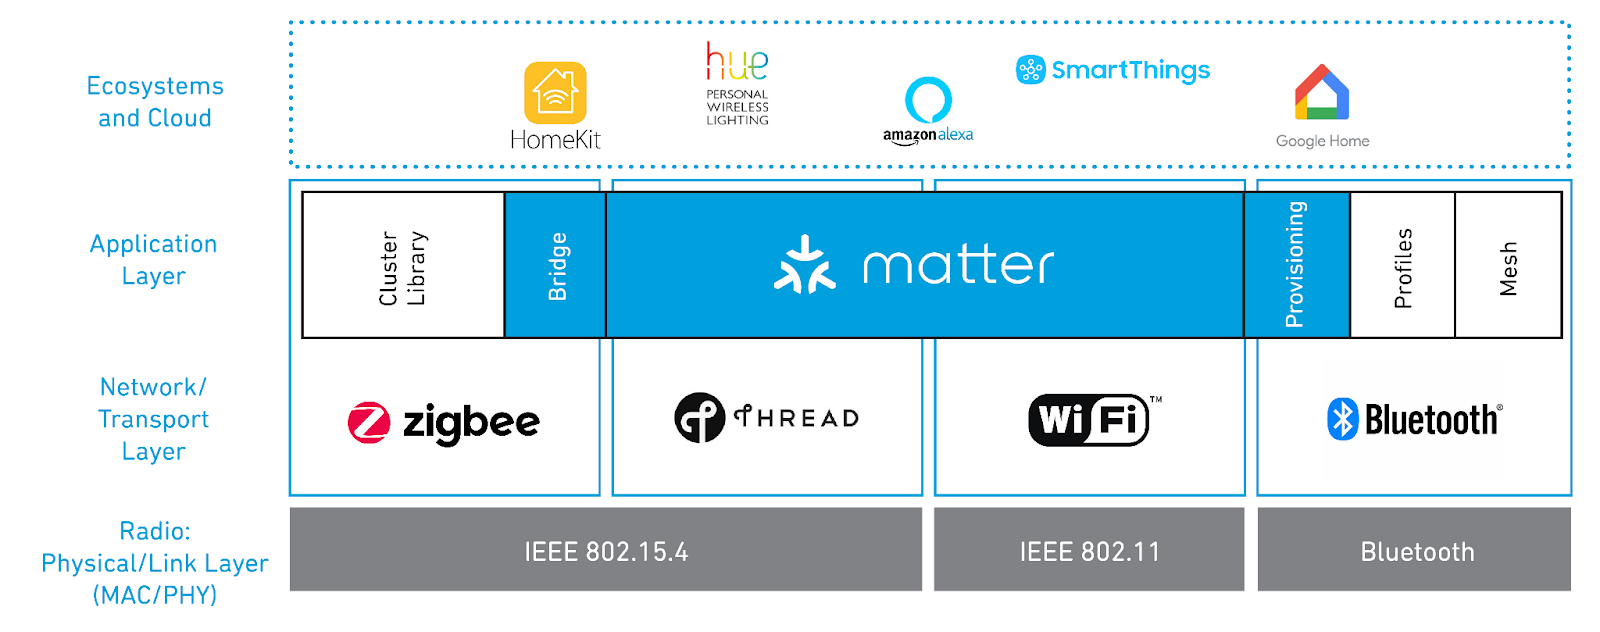
\includegraphics[width=0.9\textwidth]{DescricaoProcesso/Figuras/matter_big_arc.png}
  \caption{Arquitetura do \textit{Matter} como camada de aplicação.}
  \label{fig:matter-layer}
\end{figure}

Como descrito em \cite{matter_spec}, o protocolo Matter garante interoperabilidade entre diferentes dispositivos.

\subsection{Interface de Usuário}

A interface de usuário conecta pessoas e sistema, permitindo controle e monitoramento:

\begin{itemize}
    \item \textbf{Aplicativos Móveis e Web}: Acesso em qualquer lugar, visualização de histórico, criação de cenários e recebimento de notificações.
    \item \textbf{Painéis Físicos}: Telas sensíveis ao toque instaladas nas paredes, facilitando ajustes rápidos.
    \item \textbf{Assistentes Virtuais de Voz}: Google Assistant, Alexa, Siri, oferecendo controle sem a necessidade de interfaces gráficas.
\end{itemize}

Com o \textit{Matter}, a experiência do usuário é aprimorada, pois um único aplicativo ou assistente pode controlar dispositivos de diferentes marcas.

\subsection{Serviços em Nuvem e Análise de Dados}

A nuvem possibilita armazenamento histórico, análise avançada e integração com serviços externos:

\begin{itemize}
    \item \textbf{Análise Preditiva}: Antecipar consumos futuros, otimizar uso de energia.
    \item \textbf{Tarifas Dinâmicas}: Ajustar consumo conforme variação de preços de energia.
    \item \textbf{Manutenção Preditiva}: Identificar falhas iminentes em equipamentos.
\end{itemize}

A nuvem também permite acesso remoto, controle global e integração de APIs de terceiros, ampliando a funcionalidade do sistema.

\subsection{Segurança e Privacidade}

A crescente conectividade na automação residencial traz desafios que vão além de questões técnicas, abrangendo também a proteção de dados e o cumprimento de leis como a Lei Geral de Proteção de Dados (LGPD) no Brasil e o Regulamento Geral sobre a Proteção de Dados (GDPR) na União Europeia. Nesse contexto, é indispensável adotar medidas de segurança cibernética e garantir a privacidade dos moradores, protegendo suas informações pessoais e rotinas. O sistema deve incorporar, desde a fase de projeto, uma abordagem de \textit{Privacy by Design}, assegurando que mecanismos de proteção e conformidade estejam integrados às suas camadas mais básicas.

As principais práticas incluem:

- \textbf{Criptografia}: Todos os dados sensíveis coletados, transmitidos e armazenados devem ser protegidos por criptografia robusta, tornando-os ilegíveis a terceiros não autorizados. Assim, mesmo em caso de interceptação do tráfego de rede, informações pessoais não serão expostas, cumprindo princípios de segurança e confidencialidade exigidos pela LGPD.

- \textbf{Autenticação de Dispositivos}: Garantir que apenas dispositivos autenticados e confiáveis acessem a rede doméstica. Isso envolve a implementação de certificados digitais, chaves criptográficas ou outros métodos de autenticação forte. A restrição de acesso a dispositivos não autorizados previne usos indevidos das informações e atende aos princípios de prevenção e segurança previstos na LGPD.

- \textbf{Atualizações Seguras}: Manter o firmware dos dispositivos atualizado, corrigindo vulnerabilidades e garantindo um nível adequado de segurança contínua. O processo de atualização deve ser autenticado e seguro, impedindo que versões maliciosas sejam instaladas. Essa prática previne incidentes que possam expor dados pessoais e assegura a conformidade com a LGPD, pois reduz o risco de violações de segurança.

A privacidade é igualmente crítica. Dados sobre hábitos e rotinas dos moradores, bem como informações sobre ocupação da residência, uso de dispositivos específicos e preferências pessoais, devem ser armazenados e processados de modo a garantir o respeito à LGPD. Isso significa adotar princípios como minimização da coleta de dados (coletar apenas o indispensável para a finalidade proposta), consentimento informado dos usuários, transparência sobre como e por que os dados são usados e possibilidade de exclusão dos mesmos mediante solicitação. Além disso, todas as práticas de tratamento de dados devem estar documentadas e auditáveis, para comprovação de conformidade quando necessário.

\subsection{Integração com Outros Sistemas}

A automação residencial não funciona isoladamente. Ela pode integrar-se a sistemas de segurança, entretenimento, eletrodomésticos inteligentes e geração distribuída de energia, formando um ecossistema mais rico e funcional. Por exemplo, o sistema pode ajustar o uso de energia com base na produção solar local ou desativar determinados dispositivos ao detectar que a casa está vazia. No entanto, ao integrar múltiplos sistemas e plataformas, a complexidade na gestão dos dados aumenta. Nesse cenário, é fundamental garantir que todos os serviços externos cumpram também as normas de privacidade e segurança, incluindo a LGPD, mantendo assim a coerência e a proteção dos dados em todo o ecossistema.

\subsection{Escalabilidade e Flexibilidade}

A capacidade de crescer e se adaptar às mudanças é vital. Um sistema de automação residencial deve suportar a adição de novos dispositivos, tecnologias e serviços sem exigir reestruturações complexas. O uso de padrões abertos, como o \textit{Matter}, fortalece a escalabilidade e flexibilidade, garantindo que o sistema possa evoluir junto com o usuário e o mercado. Neste contexto, qualquer expansão deve manter o mesmo nível de conformidade com a LGPD, ampliando as práticas de segurança e privacidade para acomodar novos fluxos de dados, dispositivos e funcionalidades sem comprometer a proteção das informações pessoais.

\subsection{Instrumentação do Processo}

A instrumentação do processo envolve a seleção, instalação e configuração de sensores, atuadores e controladores. Esse cuidado na instrumentação não apenas assegura a qualidade dos dados e a efetividade das ações executadas, como também garante que o tratamento das informações coletadas obedeça aos princípios da LGPD e demais normas de proteção de dados. Para isso, alguns cuidados adicionais devem ser tomados:

- \textbf{Seleção de Hardware}: Além de atender às faixas de operação e às especificações técnicas, é importante escolher sensores e atuadores de fabricantes comprometidos com práticas adequadas de segurança e privacidade. O hardware deve permitir a implementação de criptografia, controle de acesso e atualizações seguras. Dispositivos que já seguem padrões abertos e oferecem mecanismos de proteção de dados facilitam a conformidade legal.

- \textbf{Topologia da Rede}: Ao projetar a rede, deve-se garantir cobertura de sinal, minimizar interferências e assegurar redundância em redes \textit{mesh}. Além da confiabilidade técnica, a topologia deve permitir segmentação da rede, isolando dispositivos críticos daqueles com maior risco de vulnerabilidades. Essa separação física ou lógica dificulta acessos não autorizados a dados sensíveis, contribuindo para a privacidade e segurança dos moradores.

- \textbf{Integração Elétrica}: A correta instalação elétrica, observando segurança, aterramento, fusíveis e normas técnicas, assegura não apenas o bom funcionamento dos componentes, mas também evita falhas que possam comprometer a segurança das informações. Curto-circuitos ou picos de tensão inesperados podem afetar módulos de segurança, chaves criptográficas ou até mesmo corromper dados sensíveis.

- \textbf{Provisionamento de Dispositivos}: A configuração inicial dos endereços, chaves de segurança e rotinas de atualização deve ser realizada de forma segura, garantindo que o dispositivo só seja controlado por usuários autorizados. Além disso, políticas de senhas fortes, autenticação de dois fatores e gestão de chaves criptográficas são práticas recomendadas. Essa etapa é essencial para assegurar conformidade com a LGPD, já que uma falha na configuração inicial pode resultar em acesso indevido a dados pessoais, comprometendo a privacidade dos moradores.

Em suma, a instrumentação não é apenas um aspecto técnico; ela é o alicerce para a proteção dos dados, a manutenção da segurança e o respeito à privacidade. Ao combinar boas práticas de engenharia com requisitos legais, o sistema de automação residencial pode operar de forma confiável, eficiente e em total conformidade com a LGPD e outras normas de proteção de dados.

\section{Monitoramento Energético}
\label{sec:monitoramento_energetico}

O monitoramento energético é um elemento central para a compreensão aprofundada do uso de recursos em um ambiente residencial automatizado. Mais do que simplesmente quantificar o consumo de eletricidade, o monitoramento energético permite revelar padrões, prever demandas futuras, identificar ineficiências e propor intervenções corretivas ou preventivas. Ao integrar dados provenientes de diversos sensores — incluindo aqueles dedicados à medição de corrente e tensão em circuitos específicos, bem como às tomadas e equipamentos inteligentes —, o sistema obtém uma visão holística do comportamento energético da residência.

Abaixo, são detalhadas as principais etapas e aspectos relacionados ao monitoramento energético, com especial ênfase na análise de dados, privacidade, conformidade com a LGPD, aplicações práticas e o uso de técnicas de controle estatístico de processo.
\subsection{Coleta e Organização dos Dados}

A primeira etapa do monitoramento energético consiste na coleta sistemática de dados relativos ao consumo de eletricidade em diferentes pontos da residência. Esses dados podem ser obtidos por meio de:

\begin{itemize}
    \item \textbf{Sensores de Consumo em Tempo Real}: Dispositivos que medem corrente e tensão, permitindo o cálculo instantâneo da potência e energia consumidas em circuitos específicos ou em eletrodomésticos individuais.
    \item \textbf{Tomadas e Disjuntores Inteligentes}: Elementos capazes de registrar o uso energético de um aparelho conectado, bem como ligar ou desligar o fornecimento conforme instruções do controlador.
    \item \textbf{Medição Global da Residência}: Sensores posicionados no quadro elétrico principal, fornecendo uma visão macro do consumo, contra a qual se podem comparar dados mais granulares para identificar fontes de ineficiência.
\end{itemize}

A coleta contínua gera um grande volume de dados. Para lidar com isso, é essencial adotar uma infraestrutura de armazenamento e processamento robusta. Uma opção comum é o uso de um \textbf{NAS (Network Attached Storage)}, um dispositivo de armazenamento conectado à rede local que fornece espaço centralizado e seguro para arquivamento dos dados. O NAS permite acesso controlado, backup automático e fácil ampliação da capacidade de armazenamento. Além disso, a utilização de sistemas em nuvem, servidores locais ou híbridos pode complementar o NAS, garantindo resiliência, segurança e acessibilidade dos dados.

Em qualquer cenário, devem-se implementar mecanismos de segurança (criptografia, autenticação forte) e compressão/normalização para facilitar o processamento posterior.

\subsection{Pré-Processamento, Qualidade dos Dados e Controle Estatístico de Processo}

Antes de realizar análises avançadas, os dados coletados precisam passar por etapas de pré-processamento, incluindo:

\begin{itemize}
    \item \textbf{Limpeza de Dados}: Remoção de leituras espúrias, tratamento de valores faltantes e correção de discrepâncias causadas por ruído elétrico ou falhas de comunicação.
    \item \textbf{Agregação e Granularidade}: Ajuste da escala temporal (por exemplo, sumarizar leituras segundo a segundo, minuto a minuto ou hora a hora) e espacial (agrupando dados por cômodo, circuito ou categoria de aparelho).
    \item \textbf{Normalização e Padronização}: Transformação dos dados em escalas comparáveis, permitindo análises consistentes entre diferentes pontos de medição ou períodos.
\end{itemize}

Um conjunto de dados bem pré-processado é mais coerente, confiável e adequado à aplicação de técnicas de análise estatística, aprendizado de máquina e modelagem preditiva.

Nesse contexto, o \textbf{Controle Estatístico de Processo (CEP)} pode ser aplicado ao monitoramento energético como uma ferramenta para acompanhar a variabilidade do consumo ao longo do tempo. Oriundo do domínio da qualidade industrial, o CEP utiliza gráficos de controle e limites estatísticos para distinguir variações normais de anomalias. Aplicado à automação residencial, o CEP permite:

\begin{itemize}
    \item \textbf{Estabelecer Faixas Normais de Operação}: Determinar limites superiores e inferiores para o consumo esperado, considerando padrões históricos e características da residência.
    \item \textbf{Detecção Precoce de Anomalias}: Identificar rapidamente desvios significativos, como um aumento inesperado no consumo de um aparelho, indicando falha ou uso indevido.
    \item \textbf{Monitoramento Contínuo}: Acompanhar a evolução do consumo ao longo do tempo, avaliando se as mudanças implementadas (como troca de um equipamento ou ajuste nas rotinas) resultam em maior eficiência.
\end{itemize}

O CEP atua como um complemento às técnicas de análise mais complexas, ajudando a manter o sistema dentro de parâmetros normais e fornecendo bases para intervenções pontuais.
\subsection{Análise Estatística e Inteligência Artificial}
Com dados limpos e estruturados, bem como limites estatísticos definidos pelo CEP, torna-se possível aplicar uma variedade de técnicas analíticas para extrair valor significativo:

\begin{itemize}
    \item \textbf{Estatística Descritiva}: Cálculo de médias, medianas, desvios-padrão e percentis para caracterizar o perfil de consumo energético ao longo do tempo.
    \item \textbf{Detecção de Anomalias Avançada}: Em conjunto com o CEP, métodos de aprendizado de máquina podem reconhecer padrões não lineares, detectando anomalias sutis que escapariam a métodos estatísticos convencionais.
    \item \textbf{Análise de Correlação e Causalidade}: Estabelecer relações entre o consumo energético e outras variáveis (temperatura, ocupação, eventos externos).
    \item \textbf{Modelagem Preditiva}: Uso de algoritmos de aprendizado supervisionado ou não supervisionado para prever demandas futuras, ajustar parâmetros de controle em tempo real e recomendar intervenções.
    \item \textbf{Clusterização de Perfis de Consumo}: Agrupamento de padrões de uso semelhantes, auxiliando na identificação de zonas energéticas e na otimização personalizada do sistema.
\end{itemize}

A inteligência artificial, combinada ao CEP, amplia as capacidades do sistema, tornando-o mais adaptativo e robusto. Isso resulta em ajustes proativos na operação da residência, reduzindo custos, melhorando o conforto e minimizando impactos ambientais.

\subsection{Privacidade, LGPD e Proteção dos Dados Energéticos}

As informações sobre consumo energético podem revelar hábitos, presença, rotinas e preferências dos moradores. Como tais dados podem ser considerados pessoais ou sensíveis segundo a LGPD, devem ser tratados com o mesmo rigor aplicado a outras informações coletadas:

\begin{itemize}
    \item \textbf{Minimização de Dados}: Coletar apenas o nível de detalhe necessário.  
    \item \textbf{Anonimização e Pseudonimização}: Remover ou mascarar informações identificadoras.
    \item \textbf{Consentimento e Transparência}: Explicar claramente aos moradores como, por que e por quanto tempo os dados serão coletados, analisados e armazenados.
    \item \textbf{Segurança da Informação}: Aplicar criptografia ponta a ponta, autenticação robusta e isolamento de redes.
    \item \textbf{Auditorias e Responsabilização}: Manter registros sobre o tratamento de dados, comprovando conformidade com a LGPD em caso de inspeções.
\end{itemize}

Ao equilibrar análise de dados avançada, CEP e privacidade, o monitoramento energético torna-se não apenas um recurso valioso, mas também uma solução respeitosa aos direitos e expectativas dos usuários.

\subsection{Integração com Outros Sistemas e Evolução Contínua}

O monitoramento energético não existe isoladamente. Ao integrar-se com controladores, sistemas de climatização, iluminação e segurança, bem como com serviços em nuvem e APIs externas, o sistema pode ajustar em tempo real o uso de energia conforme necessidades, demandas e condições externas.

Com a aplicação do CEP, é possível identificar se as integrações e ajustes recomendados estão mantendo o consumo dentro dos limites estatísticos esperados ou se intervenções adicionais são necessárias. Conforme novos dispositivos e tecnologias surgem, a arquitetura flexível e o uso de padrões abertos, como o \textit{Matter}, asseguram que o sistema seja escalável e possa incorporar inovações sem comprometer a segurança, a privacidade ou a qualidade da análise de dados.
\subsection{Benefícios Práticos e Responsabilidade Social}

Quando bem implementado, o monitoramento energético, aliado ao CEP e à análise de dados, traz diversos benefícios:

\begin{itemize}
    \item \textbf{Eficiência e Economia}: Redução de custos com energia elétrica por meio da identificação de desperdícios e ajustes estratégicos.
    \item \textbf{Conforto e Qualidade de Vida}: Ajustes automáticos de parâmetros ambientais conforme preferências e necessidades, sem intervenção manual constante.
    \item \textbf{Sustentabilidade}: Otimização do uso de energia, priorizando fontes renováveis e reduzindo a pegada de carbono.
    \item \textbf{Tomada de Decisão Baseada em Evidências}: Dados claros, validados e dentro de parâmetros estatísticos auxiliares guiam melhorias contínuas e embasadas em fatos.
\end{itemize}

A responsabilidade social emerge ao assegurar que tais benefícios sejam obtidos sem invadir a privacidade ou violar direitos fundamentais. A conformidade com a LGPD, o uso ético da análise de dados e a adoção de CEP garantem que a tecnologia melhore a vida dos moradores, mantendo a confiança e a proteção das informações pessoais.
Em síntese, o monitoramento energético aplicado a um sistema de automação residencial, quando embasado em um arcabouço analítico sólido, conformidade regulatória, uso de CEP e cuidado com a privacidade, transcende a mera coleta de dados. Ele estabelece um processo contínuo de aprendizado, ajuste e otimização que beneficia usuários, meio ambiente e sociedade em geral.  
\bibliography{Monografia}%,library}
\chapter{Metodologia}

Neste capítulo, são detalhadas as etapas metodológicas adotadas no desenvolvimento do sistema inteligente para monitoramento e previsão do consumo de energia residencial. A abordagem foi projetada para atender aos objetivos do projeto, combinando análise técnica, desenvolvimento de soluções e validação experimental. Os procedimentos descritos têm como objetivo garantir a reprodução, escalabilidade e eficácia do sistema proposto, contribuindo para o avanço na área de automação e eficiência energética.

\section{Pesquisa e Análise de Tecnologias Existentes}

A fase inicial do projeto consistiu na identificação e análise das tecnologias disponíveis no mercado para o monitoramento de consumo energético em residências. Esta etapa foi guiada por uma revisão bibliográfica abrangente e um estudo comparativo das soluções existentes, considerando os seguintes critérios:

\begin{itemize}
    \item \textbf{Compatibilidade com infraestruturas residenciais convencionais}: Tecnologias que não exigem modificações estruturais significativas, como sensores de fácil instalação e dispositivos autônomos.
    \item \textbf{Eficiência técnica}: Precisão na coleta de dados, robustez e confiabilidade das medições.
    \item \textbf{Interoperabilidade}: Capacidade de integração com diferentes sistemas e protocolos, como Wi-Fi, Zigbee e Bluetooth Low Energy.
    \item \textbf{Custo-benefício}: Viabilidade econômica para implementação em larga escala.
\end{itemize}

A análise resultou na seleção de componentes que atendem aos requisitos do projeto. Foi escolhida a linha de tomadas \textit{Tuya Smart Wi-Fi}, cuja modularidade permite fácil instalação em diversos locais, utilizando a metodologia \textit{plug and play}. Estas tomadas oferecem integração com a plataforma \textit{Tuya Cloud} e suas APIs, garantindo flexibilidade e escalabilidade.

\section{Desenvolvimento do Protótipo}

Com base nas tecnologias identificadas, foi desenvolvido um protótipo funcional que integra hardware e software para monitoramento e previsão de consumo energético. O desenvolvimento seguiu as seguintes etapas:

\subsection{Seleção e Configuração de Sensores}

As tomadas \textit{Tuya Smart Wi-Fi} foram configuradas para monitorar o consumo energético em tempo real. Estes dispositivos enviam os dados para a plataforma \textit{Tuya Cloud}, de onde são acessados por meio de APIs.

\subsection{Desenvolvimento do Sistema de Controle}

O sistema de controle foi desenvolvido utilizando as APIs fornecidas pela \textit{Tuya Cloud}, permitindo a comunicação entre as tomadas e o sistema central. O controlador é responsável por:

\begin{itemize}
    \item Receber e processar os dados coletados pelas tomadas.
    \item Aplicar algoritmos de análise e previsão de consumo.
    \item Integrar os dados a uma interface de visualização desenvolvida especificamente para o projeto.
\end{itemize}

\subsection{Desenvolvimento da Interface de Visualização}

A interface de monitoramento foi desenvolvida pelo autor do trabalho utilizando linguagens de programação voltadas para desenvolvimento web e visualização de dados. Esta interface exibe de forma intuitiva os padrões de consumo energético, permitindo que os usuários identifiquem desperdícios e ajustem seu comportamento para otimizar o uso de energia.

\section{Implementação de Algoritmos de Processamento e Previsão}

Para o tratamento dos dados coletados, foram desenvolvidos e implementados algoritmos específicos, detalhados a seguir:

\subsection{Pré-processamento dos Dados}

Os dados brutos coletados pelas tomadas passaram por etapas de limpeza e normalização, eliminando leituras espúrias e garantindo consistência nos resultados.

\subsection{Análise Estatística e Controle Estatístico de Processos (CEP)}

O CEP foi utilizado para identificar variações significativas no consumo energético, estabelecendo limites de controle e detectando anomalias. Esta abordagem foi complementada por métodos estatísticos descritivos para caracterizar os padrões de consumo.

\subsection{Previsão de Consumo com Inteligência Artificial}

Modelos de aprendizado de máquina foram treinados utilizando dados históricos para prever demandas futuras de energia. Técnicas como regressão linear e redes neurais foram aplicadas, visando maior precisão e adaptabilidade.

\section{Validação em Ambiente Real}

O protótipo foi testado em um ambiente residencial que não possuía infraestrutura prévia de automação. A validação envolveu:

\begin{itemize}
    \item \textbf{Avaliação de desempenho}: Testes para verificar a precisão das tomadas \textit{Tuya Smart Wi-Fi} e a eficiência dos algoritmos.
    \item \textbf{Usabilidade}: Análise da interface para garantir que usuários finais pudessem interpretar os dados facilmente.
    \item \textbf{Robustez}: Monitoramento contínuo em condições reais, avaliando a resiliência do sistema a falhas.
\end{itemize}

Os resultados dos testes foram documentados e utilizados para refinar o sistema, corrigindo inconsistências e melhorando sua eficiência.

\section{Viabilidade de Implementação em Larga Escala}

A análise de viabilidade considerou aspectos técnicos, econômicos e sociais, como:

\begin{itemize}
    \item \textbf{Custos de produção}: Avaliação dos investimentos necessários para replicação do sistema.
    \item \textbf{Benefícios econômicos}: Potencial de redução de custos para os usuários com base na diminuição do desperdício energético.
    \item \textbf{Impactos ambientais}: Contribuição para a sustentabilidade por meio do uso eficiente de energia.
    \item \textbf{Estratégias de adoção}: Identificação de barreiras e propostas para ampliar o alcance do sistema, como parcerias com fabricantes de dispositivos inteligentes.
\end{itemize}

\section{Resumo do Capítulo}

Este capítulo detalhou as etapas metodológicas seguidas no desenvolvimento do sistema inteligente para monitoramento e previsão de consumo de energia residencial. As etapas compreenderam a análise de tecnologias, desenvolvimento do protótipo utilizando as tomadas \textit{Tuya Smart Wi-Fi}, implementação de algoritmos avançados, validação experimental e estudo de viabilidade em larga escala. A abordagem proposta combina rigor técnico e aplicabilidade prática, destacando-se como uma solução promissora para o setor de automação residencial.
\chapter{Resultados}

Para a execução do projeto, algumas etapas de desenvolvimento tiveram de ser seguidas: familiarização com o sistema, estudo dos módulos envolvidos, leitura dos requisitos, elaboração de documento descrevendo todo o processo de implementação e relacionamento com os diversos módulos, implementação e testes.


\section{Atividades do Projeto}
\label{metodo3}

\section {Requisitos do Sistema}
\label{req}


\section{Desenvolvimeto e Implementação}

A Tabela \ref{tab:tabela} apresenta as atividades executadas.

\begin{table}
\centering
%Note os alinhamentos diferentes em cada coluna
\begin{tabular}{|c|r|l|}\hline
		Atividade 1 & aa  & ab  \\ 
					 & a & b \\ \hline
		Ativ. 2  & aa & ab \\			
					 &  a & b \\ \hline
		\end{tabular}
	\caption{Exemplo de tabela - Coloque toda informação sobre a tabela aqui}
	\label{tab:tabela}
\end{table}

\section{Testes}

\section{Análise dos Resultados}

Apresente os resultados sem adulterações e faça análises objetivas. Pense na melhor maneira de apresentar os resultados graficamente. Se os gráficos são difíceis de interpretar, talvez tabelas sejam uma forma melhor de apresentar resultados. Não apresente dados (gráficos e tabelas) se não há uma conclusão interessante a ser tirada. Lembre-se de ser conciso.

\emph{Não se esqueça das unidades!} Pense que \emph{a priori} todo número deve ter uma unidade. Não escreva as unidades em itálico (no ambiente matemático) e tome cuidado para diferenciar maiúsculas e minúsculas. Um exemplo é escrever $22$ [kN] e não $22 KN$ (Kelvin vezes Newton!).

Ao apresentar resultados experimentais, tome o cuidado para também apresentar o cálculo das incertezas sempre que forem significativas. Ao fazer conclusões, sempre considere se o tamanho da sua amostra é grande o suficiente do ponto de vista estatístico. Lembre que a média empírica $\hat{\mu}_X$ de $N$ observações independentes da variável $X_i$ possui variância
\[
\hat{\sigma}_{\mu}^2 = \frac{1}{N(N-1)} \sum_{i=1}^N (X_i-\hat{\mu}_X)^2
\enspace,
\]
onde se assume que as variáveis $X_i$ possuem uma mesma ditribuição e que essa distribuição possui segundo momento finito.


\section{Resumo do Capítulo}
\label{sec:resumoo4}
Tente não terminar de forma abrupta. Se for escrever algo aqui, não seja genérico!

\section{Formato, expressões matemáticas e o \LaTeX}

\subsection{O \LaTeX}

O {\LaTeX}  é o método preferencial de preparação de documentos para textos técnicos nas ciências exatas. O {\LaTeX} permite não só lidar com equações de uma forma mais prática que em editores de texto, mas também facilita a formatação de documentos e tem um desempenho marcadamente superior a editores de texto na preparação de documentos longos como monografias. 

Documentos em {\LaTeX} são escritos em um ou mais arquivos de texto com extensão .tex. Após a escrita, o .tex é \emph{compilado} para gerar arquivos nos formatos .pdf, .dvi ou .ps. Hoje há duas distribuições padrão para o \LaTeX. Sistemas Windows usam o {Mik\TeX} e sistemas Unix usam o \TeX Live. Além das distribuições, muitos usuários utilizam \emph{front-ends} que facilitam a edição do texto, a compilação e a instalação de pacotes. 

Os pacotes necessários para compilar o presente documento devem ser encontrados numa instalação completa dessas distribuições. Se tiver dificuldades com os pacotes, você pode instalá-los manualmente ou tentar alterar o código para usar versões antigas dos mesmos.

A compilação pode ser feita pelos comandos \textsf{latex} ou \textsf{pdflatex}, invocados pela linha de comando ou pelo \emph{front-end}. Note que será necessário empregar o comando \textbf{mais de uma vez} para que as referências cruzadas saiam corretas.

Como discutido na Seção \ref{sec:revisão}, uma ferramenta útil para gerenciar as citações em {\LaTeX} é o Bib\TeX. Para gerar uma lista bibliográfica a partir do arquivo .bib, este arquivo deve ser indicado no arquivo .tex. Em seguida devem-se executar os comandos \textsf{pdflatex}, \textsf{bibtex} e \textsf{pdflatex} novamente sempre usando o .tex como argumento. Note que os comandos são executados nesta ordem e de forma repetida para que as referências cruzadas sejam geradas corretamente.

Nesta seção você deve encontrar exemplos dos comandos mais usados em \LaTeX. Outros exemplos e manuais podem ser encontrados na internet com facilidade.

\subsection{Expressões Matemáticas}

Ao escrever expressões matemáticas, defina todas as variáveis antes de usá-las ou imediatamente depois da expressão. Deixar de fazê-lo torna seu texto \textbf{ilegível}. Segue um exemplo.

Seja o par $(a_1,a_2)\in \mathbb{R}^2$. Para $s\in\mathbb{C}$, definimos a função $f(s)$ como
\[%cria equações sem numeração
f(s)\triangleq \frac{a_1 s+a_2}{s^2+2\zeta\omega_n s+\omega_n^2}
\enspace,
\]
onde os escalares $\zeta,\omega_n>0$ são constantes.

Note que não foi necessário atribuir valores às variáveis neste momento. Repare também como devemos \textbf{usar pontuação} (vírgula) nas equações, tratando-as como parte da frase. Usamos o símbolo $\triangleq$ ou $:=$ para deixar explícito que se trata de uma definição. Ser claro nesse aspecto facilita o entendimento do leitor.

A equação acima não foi numerada porque não será citada no texto. Vejamos um exemplo com numeração.

A função $f(\cdot)$ possui um zero em $-a_2/a_1$ (ou $-\frac{a_2}{a_1}$) e, para $\zeta<1$, possui polos complexos $p_{1,2}$ dados por
\begin{equation}
\label{eq:polos}
p_{1,2}=\omega_n \left(-\zeta\pm j\sqrt{1-\zeta^2}\right)
\enspace.
\end{equation}
Agora podemos citar os polos dados pela Equação (\ref{eq:polos}) (aqui adotamos a convenção de citar sempre com o número entre parênteses precedido da palavra Equação). Note como usamos um comando especial na Equação \ref{eq:polos} para garantir o ajuste automático do tamanho dos parênteses.

Vejamos agora como criar equações alinhadas. Considere o sistema dinâmico dado pelas equações diferenciais:

\begin{align}
\dot{x}_1 & = \cos(x_2)\cdot\ln(1/x_1)+\tan(u) \label{eq:x1dot} \\
\dot{x}_2 & = e^{-x_1-x_2} \nonumber \\
& y  = \min\{x_1,x_2\}  \label{eq:saida}
\enspace,
\end{align}
onde $x(t)=[x_1(t) ~ x_2(t)]'$, $t>0$, é a variável de estado do sistema, $u(t)$ é o sinal de entrada e $y(t)$ é o sinal de saída do sistema. Note no .tex que o caracter de tabulação \textsf{\&} foi usado para indicar o ponto de alinhamento horizontal das equações. Além disso, para ilustrar o uso do \LaTeX, retiramos a numeração da segunda equação e citamos as equações separadamente.

Nas Equações (\ref{eq:x1dot}) e (\ref{eq:saida}), aparecem operadores como $\min$, $\ln$, $\cos$ e $\tan$. A convenção aqui é que \textbf{variáveis devem ser escritas em itálico e operadores não}. Por essa razão todas as expressões matemáticas devem ser escritas no ambiente matemático (entre cifrão) mesmo quando for possível usar texto comum. Isso garante a consistência das fontes utilizadas (nem sempre a fonte do ambiente matemático é a mesma fonte do texto). 

Para escrever matrizes, podemos fazer por exemplo:
\[
\sum_{n=0}^{\infty}z^{-n}\left[\begin{array}{cc}
\lambda & 1 \\
0 & \lambda
\end{array}\right]^n=
\left[\begin{array}{cc}
\frac{z}{z-\lambda} & \frac{z}{(z-\lambda)^2} \\
0 & \frac{z}{z-\lambda}
\end{array}\right]
,~\forall \lambda<|z|
\enspace.
\]

Para escrever uma expressão com múltiplos casos, podemos fazer, para um inteiro $N$ positivo,
\[
g[n]=
\left\{
\begin{array}{ll}
0,& \mbox{se }~ n\leq 0 \\
n,& \mbox{se }~ n=1,2,\ldots,N-1 \\
N,& \mbox{se }~ n\mod N = 0 \\
0,& \mbox{caso contrário}\enspace.
\end{array}
\right.
\]

\textbf{Nunca reaproveite símbolos} matemáticos, isto é, nunca use o mesmo símbolo para designar variáveis diferentes.

Para um exemplo com múltiplas linhas de expressão matemática: tem-se que, para $a\neq 0$,

\begin{equation}
\begin{split}
ax^2+bx+c &= 0 \\
& \Rightarrow a(x^2+bx/a+c/a) =0 \Rightarrow a((x+b/(2a))^2+c/a-b^2/(4a^2))=0  \\
& \Rightarrow (x+b/(2a))^2=(b^2-4ac)/(4a^2) \\
& \Rightarrow (x+b/(2a))=\pm\sqrt{b^2-4ac}/(2a) \\
& \Rightarrow x=\frac{-b\pm\sqrt{b^2-4ac}}{2a}
\enspace.
\end{split}
\end{equation}

Note a argumentação lógica aqui. Não estamos dizendo que o valor de $x$ é dado pela última linha. Estamos dizendo que a hipótese da primeira linha juntamente com a hipótese $a\neq 0$ implicam os referidos valores de $x$. \textbf{Um erro comum dos alunos ao escrever é não distinguir a veracidade das implicações com a veracidade das hipóteses}.

\clearpage
\chapter{Conclusões}

Novamente, este será um dos trechos que o leitor experiente lerá antes de decidir se vale a pena ler o texto integral. Seja convincente.

\section{Considerações Finais}

Reitere o que de mais importante foi feito, qual era o objetivo inicial e qual o resultado obtido. Se houve requisitos ou especificações de projeto, discuta se foram atingidos. Se os resultados não foram conclusivos ou contrariam o que se esperava, seja honesto e diga-o explicitamente. Busque explicar os insucessos com argumentos sólidos e plausíveis. 

\section{Propostas de Continuidade}

Se houve questões ainda não respondidas ou resultados insatisfatórios, aponte direções de continuação.

\clearpage


\addcontentsline{toc}{chapter}{Referências Bibliográficas}
\renewcommand{\bibname}{Referências Bibliográficas}

%\bibliographystyle{abntex2-alf} %para norma ABNT no sistema autor-data
\bibliographystyle{abntex2-num}
\begin{small}
\bibliography{ListadeReferencias}%,library}
%% Monografia para Projeto de Fim de Curso - Exemplo no LaTeX
%-----------------------------------------------------------


%---------------Inicialização de pacotes--------------------

\documentclass[12pt,a4paper,notitlepage,twoside]{book}


\usepackage{graphicx}
\usepackage[utf8]{inputenc}
%\usepackage[latin1]{inputenc} %%pode ser necessário trocar a codificação em sistemas Windows
\usepackage[brazil]{babel}		%%pode ser necessário trocar o pacote de línguas em algumas distribuições LateX
%\usepackage[portuguese]{babel}
\usepackage[T1]{fontenc}
\usepackage{amsmath,amssymb}
\usepackage{amsthm,amsfonts}
\usepackage{color}
\usepackage[colorlinks]{hyperref}
\usepackage{abntex2abrev}
%\usepackage[alf]{abntex2cite} %se você quiser seguir as normas ABNT no sistema autor-data
%\usepackage[num]{abntex2cite} %se você quiser seguir as normas ABNT no sistema numérico
\usepackage{setspace}
\usepackage[toc,page]{appendix}

%Definindo fonte Times (Use os pacotes obsoletos se não conseguir instalar os atualizados)
%\usepackage{times}     %Pacote de fontes obsoleto, apenas texto
%usepackage{mathptmx}  %Pacote de fontes obsoleto, texto e símbolos matemáticos
%\usepackage{newtxtext,newtxmath}  %Pacotes de fontes mais recentes

\usepackage[a4paper,top=30mm,bottom=30mm,inner=30mm,outer=25mm,headheight=7mm,headsep=6mm,footskip=7mm]{geometry}
\usepackage{enumerate}

\makeindex

%\singlespacing   %%espaçamento simples
%\onehalfspacing
%\setstretch{1.03} %%um pouco melhor que espaçamento simples
\linespread{1.25} %corresponde ao espaçamento 1.5 do MS Word

%---------------Início do documento-------------------------

\begin{document}

\begin{titlepage}
\begin{center}
{\large Universidade Federal de Minas Gerais\\
Escola de Engenharia \\
Curso de Graduação em Engenharia de Controle e Automação\\}

\vspace{6cm}
{\bf\Large Monitoramento e previsão do consumo de energia residencial baseado em Sistemas
Inteligentes\vspace{0.2cm}}

\vspace{4cm}

%\hspace{0.3\textwidth} \parbox{0.65\textwidth}
{\large Igor Cleto Silva de Araújo}
\vspace{2cm}  
   
\vspace{2cm}          
%\hspace{0.3\textwidth} 
{\large Orientadora: Prof Carmela Maria Polito Braga}\\

\vfill
%\hspace{0.3\textwidth} 
{\large Belo Horizonte, Outubro de 2024 }
\end{center}

\end{titlepage}

\newpage
\clearpage
\thispagestyle{empty}


\begin{titlepage}

\centering
\textbf{Monografia}\\
\vspace{2cm}
\centering
\textbf{Monitoramento e previsão do consumo de energia residencial baseado em Sistemas
Inteligentes}\\
\vspace{5cm} 

\parbox{1.0\textwidth} 
{\large 
Monografia submetida à banca examinadora
designada pelo Colegiado Didático do Curso de
Graduação em Engenharia de Controle e
Automação da Universidade Federal de Minas
Gerais, como parte dos requisitos para aprovação na
atividade Projeto Final de Curso II.}

\vspace{7cm} 
\centering
Belo Horizonte, Outubro de 2024

\end{titlepage}


\pagenumbering{roman}
\addcontentsline{toc}{chapter}{Resumo}

\begin{center}
\huge{{\bf Resumo}}
\vspace{2cm}
\end{center}

No Resumo, em uma única página, em no máximo dois parágrafos, você explicita os seguintes itens: objetivos do projeto e descrição sucinta do local onde ele foi desenvolvido; metodologia utilizada; e resultados alcançados. Leitores experientes decidem se prosseguirão para a leitura do texto completo após lerem o resumo, a conclusão e a introdução. Por isso nestes lugares você deve colocar um esforço maior de convencimento. Além disso, a linguagem utilizada deve ser acessível a leitores com pouca familiaridade com a área, limitando-se o uso de jargões.
 
\begin{sloppypar}
Este novo parágrafo serve para mostrar que ao pular uma ou mais linhas no texto do arquivo .tex, o \TeX\ entende que você está iniciando outro parágrafo. O comando \textsf{sloppypar} força o texto a não ultrapassar as margens. Só deve ser usado se este problema ocorrer.
\end{sloppypar}

 
\clearpage
\thispagestyle{empty}
\cleardoublepage


\addcontentsline{toc}{chapter}{Abstract}

\begin{center}
\huge{{\bf Abstract}}
\vspace{2cm}
\end{center}

This project aims to develop an intelligent system for monitoring and forecasting energy consumption in homes that were not originally designed for home automation. Specifically, it seeks to research and analyze existing technologies that allow energy monitoring without requiring prior infrastructure, and to explore solutions suitable for conventional residences. The project will involve the development of a prototype for an easily installable and user-friendly monitoring system, as well as the implementation of data processing algorithms and consumption forecasting using artificial intelligence techniques. An intuitive software platform will be created for users to visualize and analyze the data, and the system will be tested and validated in a real-world environment to ensure its efficiency and usability. To promote the feasibility of large-scale implementation, the project will include cost analysis and strategies for adoption. Finally, the results will be documented and disseminated, emphasizing the contributions to Control and Automation Engineering and the social and environmental benefits provided by the developed system. 

\clearpage
\thispagestyle{empty}
\cleardoublepage


\addcontentsline{toc}{chapter}{Agradecimentos}

\begin{center}
\huge{{\bf Agradecimentos}}
\vspace{4cm}
\end{center}

Gostaria de expressar minha profunda gratidão a Deus, pela saúde física e mental que me permitiu a realização dos meus sonhos e objetivos. Aos meus pais, meu sincero agradecimento pelo suporte incondicional aos meus estudos desde a minha infância, sempre acreditando em meu potencial e me incentivando a seguir em frente. Agradeço também aos meus professores e gestores, que, com seu apoio e ensinamentos, tanto dentro quanto fora da sala de aula, contribuíram para a minha formação acadêmica e pessoal. Não poderia deixar de agradecer, de maneira especial, à minha orientadora, Profª. Carmela Maria Polito Braga, pela dedicação, paciência e orientação ao longo deste um ano de desenvolvimento deste trabalho. Sua contribuição foi fundamental para a realização deste projeto. A todos, meu muito obrigado.
 
\clearpage
\thispagestyle{empty}
\cleardoublepage
\tableofcontents
%\markboth{Conteúdo}{Conteúdo}

\clearpage
%\thispagestyle{empty}
%\cleardoublepage

% Normalmente, este arquivo só contém isto.
\listoffigures
\addcontentsline{toc}{chapter}{Lista de Figuras}
%\markboth{Lista de Figuras}{Lista de Figuras}

\clearpage
%\thispagestyle{empty}
%\cleardoublepage

% Normalmente, este arquivo só contém isto.
\listoftables
\addcontentsline{toc}{chapter}{Lista de Tabelas}
%\markboth{Lista de Tabelas}{Lista de Tabelas}

\clearpage
%\thispagestyle{empty}
%\cleardoublepage

% Normalmente, este arquivo só contém isto.

\pagenumbering{arabic}
\setcounter{page}{1}
\chapter{Introdução}
\label{chap:intro} %este label será usado para referenciar este capítulo

% As primeiras frases têm a missão de prender a atenção do leitor e por isso são as mais importantes do texto. Diga o quanto antes o que você fez e quais são os resultados alcançados. Ao terminar de ler a introdução o leitor tomará uma nova decisão de se vale a pena ou não continuar lendo o texto. Capte a atenção do leitor bem aqui.

% A comunicação escrita é considerada umas das cinco habilidades mais importantes por profissionais de engenharia e um engenheiro passa em média mais de $25$\% do seu tempo escrevendo \cite{eggert2002response,spretnak1982survey}. Uma quantidade similar de tempo é gasta na escrita de correspondência e de relatórios técnicos \cite{cunningham2012perceptions}. Dessa forma, encare a escrita do seu projeto como um treinamento nessa importante habilidade.

% Neste texto você encontrará não apenas uma estrutura para escrever seu trabalho em \LaTeX, mas também um pequeno manual de boas práticas na escrita técnica. Leia com atenção e coloque as sugestões em prática à medida que preenche o texto com o conteúdo do seu próprio projeto. Também será apresentado um número de vícios de escrita comumente encontrados nas monografias de alunos. 

% A seguir está a estrutura de organização sugerida pelo colegiado do curso. Note que ela não é necessariamente a melhor para contar a história do seu projeto. Você pode por exemplo preferir usar títulos mais pertinentes ao seu contexto. Contudo, o seu texto deve conter cada um dos pontos a seguir.

\section{Motivação e Justificativa}
\label{sec:motivacao}

A crescente demanda por energia elétrica, aliada à necessidade de uso eficiente dos recursos energéticos, torna imperativo o desenvolvimento de soluções inovadoras que permitam aos consumidores monitorar e gerenciar seu consumo de forma eficaz e em tempo real. No contexto residencial, muitas vezes os usuários não têm acesso a informações detalhadas sobre o consumo energético em suas casas, o que dificulta a identificação de desperdícios e a implementação de medidas para a redução do consumo. O cenário se agrava devido à falta de sistemas acessíveis e de fácil implementação para o monitoramento eficiente, o que resulta em uma grande dificuldade para os consumidores em adotar práticas mais sustentáveis e econômicas no seu cotidiano. 

Além disso, a automação residencial enfrenta desafios consideráveis relacionados à integração de dispositivos e sensores de diferentes fabricantes. A grande diversidade de tecnologias, protocolos de comunicação e padrões de mercado, somada à ausência de uma padronização efetiva entre os diferentes fabricantes, cria um ambiente no qual os dispositivos muitas vezes não se comunicam de maneira eficiente, impedindo a criação de sistemas unificados de monitoramento e controle. Esse cenário limita os benefícios da automação, como a otimização do consumo de energia e a melhoria da qualidade de vida dos moradores, além de dificultar o acesso a tecnologias que poderiam proporcionar um ambiente mais confortável, seguro e sustentável.

Adicionalmente, muitas residências não foram originalmente projetadas com infraestrutura para automação, o que torna a adaptação desses ambientes ao uso de tecnologias de monitoramento e controle mais complexa e dispendiosa. A implementação de soluções de automação, frequentemente, exige modificações estruturais significativas, que podem tornar o processo oneroso e inviável para uma grande parcela da população. Isso, por sua vez, desencoraja muitos proprietários a adotarem essas tecnologias, deixando uma significativa quantidade de residências sem os benefícios em termos de eficiência energética, conforto e segurança que poderiam ser proporcionados por sistemas de automação. Assim, a falta de alternativas acessíveis e de fácil implementação para o monitoramento e gestão do consumo energético representa uma grande oportunidade de desenvolvimento de soluções que possam superar essas barreiras técnicas e financeiras e beneficiar uma ampla gama de usuários.

\section{Objetivos do Projeto}
\label{sec:objetivos}

Tendo em vista o exposto acima, este projeto tem por objetivos:

\begin{enumerate}[a)]
\item Realizar uma pesquisa e análise de tecnologias existentes que permitam o monitoramento energético sem a necessidade de infraestrutura prévia;
\item Explorar soluções adequadas para residências convencionais, que não foram originalmente projetadas para automação residencial;
\item Desenvolver um protótipo de sistema de monitoramento de fácil instalação e uso;
\item Implementar algoritmos de processamento de dados e previsão de consumo utilizando técnicas de inteligência artificial;
\item Criar uma plataforma de software intuitiva para visualização e análise dos dados pelos usuários;
\item Testar e validar o sistema em ambiente real, garantindo sua eficiência e usabilidade;
\item Promover a viabilidade de implementação em larga escala por meio da análise de custos e estratégias de adoção;
\item Documentar e divulgar os resultados obtidos, destacando as contribuições para a Engenharia de Controle e Automação e os benefícios sociais e ambientais proporcionados pelo sistema desenvolvido.
\end{enumerate}

\section{Local de Realização}
\label{sec:empresa}

O local de realização deste projeto é a residência do próprio desenvolvedor, onde os testes dos equipamentos e a simulação das necessidades reais de automação residencial estão sendo realizados. A escolha deste ambiente se justifica pela possibilidade de realizar uma avaliação prática e realista das soluções de monitoramento e previsão de consumo energético, simulando as condições do dia a dia em uma residência convencional. A residência não foi originalmente projetada com infraestrutura para automação, o que representa um desafio adicional, mas também um aspecto relevante para a validação do sistema, pois permite testar a adaptação de tecnologias em um ambiente que não conta com recursos avançados de automação.

Neste contexto, o projeto visa avaliar a viabilidade de implementação de soluções de monitoramento energético em ambientes residenciais que, assim como muitas casas, não foram concebidos para suportar sistemas automatizados. Dessa forma, o projeto busca não apenas desenvolver uma solução eficiente, mas também uma que seja de fácil adaptação e acessível para a grande maioria dos consumidores. O vínculo com o local de testes é direto, pois, além de ser o ambiente de realização das simulações, a residência do desenvolvedor também serve como um campo de experimentação e validação para os resultados do sistema proposto.

\section{Estrutura da Monografia}
\label{sec:organizacao}

O trabalho está dividido em quatro capítulos. Este capítulo apresentou uma introdução ao projeto descrito nesta monografia, incluindo o objetivo de desenvolvimento de um sistema inteligente para monitoramento e previsão de consumo de energia em residências, além de descrever o local de realização dos testes, que ocorre na residência do próprio desenvolvedor. O Capítulo 2 descreve os princípios básicos de um sistema de automação residencial e monitoramento energético, abordando todos os conceitos necessários para um melhor entendimento do projeto. O Capítulo 3 explora a metodologia de desenvolvimento, incluindo a análise das tecnologias existentes, a criação do protótipo e a implementação dos algoritmos de processamento de dados e previsão de consumo. No Capítulo 4, apresenta-se a conclusão da monografia, com um resumo dos resultados alcançados e algumas sugestões e dificuldades encontradas durante a realização do projeto.

\clearpage
\chapter[Princípios de Automação Residencial]{Princípios básicos de um sistema
de automação residencial e monitoramento energético}
\label{chap:principios}
%Note que, como o nome do capítulo é muito longo, fornecemos um nome abreviado para uso no cabeçalho

Este capítulo apresenta uma visão abrangente dos princípios fundamentais na concepção, implementação e operação de um sistema inteligente de automação residencial orientado ao monitoramento e previsão do consumo energético. O contexto abordado parte da realidade de residências convencionais, isto é, aquelas que não dispõem de infraestrutura prévia de automação, exigindo assim soluções flexíveis, escaláveis e capazes de integrar múltiplos dispositivos e tecnologias. Nosso enfoque não se limita ao simples acionamento de equipamentos, mas abrange a coleta e análise detalhada de dados, permitindo uma gestão mais eficiente dos recursos, redução de custos, melhoria do conforto e incremento da sustentabilidade ambiental.

Iniciamos com um exame minucioso da arquitetura típica de um sistema de automação residencial, descrevendo os principais componentes: sensores (ambientais, de presença, de consumo energético), atuadores (termostatos, dimmers, motores para cortinas, entre outros), controladores (centralizados e distribuídos), protocolos de comunicação (Wi-Fi, Zigbee, Z-Wave, BLE, Thread e \textit{Matter}) e interfaces de usuário (aplicativos, painéis físicos, assistentes de voz). Destacamos, em especial, o \textit{Matter}, um protocolo emergente que unifica e facilita a interoperabilidade entre dispositivos de diferentes fabricantes, garantindo flexibilidade, segurança e escalabilidade ao ecossistema doméstico conectado.

Em seguida, detalhamos o processo de instrumentação do sistema, abordando a seleção criteriosa de hardware, a integração de sensores e atuadores, bem como a definição da topologia da rede. Esse cuidado assegura a qualidade dos dados coletados, a robustez do controle e a adequação às normas legais. A segurança da informação e a privacidade são tratadas de forma transversal, observando-se os princípios da Lei Geral de Proteção de Dados (LGPD) e adotando medidas como criptografia, autenticação de dispositivos, minimização de dados e consentimento informado dos usuários.

Outro ponto central é o monitoramento energético. Não se trata apenas de registrar o consumo, mas de transformar dados brutos em conhecimento. São exploradas técnicas de pré-processamento, análise estatística, aprendizado de máquina e Controle Estatístico de Processo (CEP) para detectar anomalias, identificar padrões de consumo, antecipar demandas e propor intervenções que otimizem o uso de energia. Essas abordagens analíticas embasam decisões proativas, possibilitando desde ajustes automáticos de cargas elétricas até a recomendação de substituição de equipamentos ineficientes, o que resulta em benefícios econômicos, maior conforto e redução do impacto ambiental.

Ao compreender as soluções existentes, suas limitações e potenciais, este capítulo fornece uma base sólida para os desenvolvimentos subsequentes, orientando tanto a implementação prática do protótipo quanto a evolução do sistema no sentido de maior inteligência, integração e respeito à privacidade e às leis vigentes.

\section{Arquitetura de um Sistema de Automação Residencial}

A arquitetura de um sistema de automação residencial é composta por diversos elementos que trabalham em conjunto para oferecer controle, monitoramento e otimização de aspectos como eficiência energética, segurança, conforto e conveniência. Ela não consiste apenas em dispositivos isolados, mas em um ecossistema integrado capaz de entender as condições do ambiente, agir de forma proativa e se adaptar às preferências dos moradores.

A seguir, detalhamos os principais elementos dessa arquitetura, estabelecendo as bases para compreender as complexidades e potencialidades de tais sistemas.

\subsection{Sensores}

Os sensores representam a interface entre o mundo físico e o digital. Eles coletam dados sobre o ambiente e o estado dos dispositivos, fornecendo informações essenciais para que o sistema possa tomar decisões informadas. Podem monitorar temperatura, umidade, luminosidade, qualidade do ar, presença de pessoas e consumo de energia, entre outros parâmetros. Alguns exemplos:

\begin{itemize}
    \item \textbf{Sensores de movimento e presença}: Utilizam tecnologias como infravermelho passivo (PIR), ultrassom ou micro-ondas. Além de acionar luzes ou alarmes, podem colaborar na climatização, ajustando a temperatura apenas em ambientes ocupados.
    \item \textbf{Sensores ambientais (temperatura, umidade, qualidade do ar)}: Auxiliam no controle de sistemas de HVAC (Aquecimento, Ventilação e Ar Condicionado), garantindo conforto térmico e qualidade do ar interno.
    \item \textbf{Sensores de luminosidade}: Ajustam iluminação artificial conforme a luz natural, otimizando o uso de energia e melhorando o bem-estar.
    \item \textbf{Sensores de consumo energético}: Medem o consumo de dispositivos específicos ou circuitos, fornecendo dados granulares para análise, detecção de aparelhos ineficientes e implementação de estratégias de economia de energia.
\end{itemize}

A seleção e instalação adequadas dos sensores são fundamentais, influenciando a qualidade dos dados coletados e a efetividade das estratégias de controle.

\subsection{Atuadores}

Atuadores transformam as decisões do sistema em ações físicas. Podem ser relés, motores, dimmers ou válvulas controladas eletronicamente, acionando iluminação, climatização, cortinas, persianas, eletrodomésticos e outros dispositivos.

\begin{itemize}
    \item \textbf{Interruptores e dimmers inteligentes}: Ligam, desligam ou ajustam a intensidade luminosa, criando cenários adequados para diferentes atividades.
    \item \textbf{Termostatos inteligentes}: Regulam o aquecimento ou resfriamento, aprendendo rotinas e antecipando demandas, reduzindo custos e melhorando o conforto.
    \item \textbf{Motores para cortinas e persianas}: Controlam entrada de luz e calor, integrando-se a sensores de luminosidade e temperatura para otimizar a eficiência energética.
    \item \textbf{Tomadas inteligentes}: Permitem ligar e desligar aparelhos remotamente, fornecendo dados de consumo e contribuindo para reduzir o uso excessivo de energia.
\end{itemize}

A qualidade, confiabilidade e responsividade dos atuadores são essenciais para garantir que as decisões do sistema sejam efetivamente postas em prática.

\subsection{Controladores}

Os controladores são o “cérebro” do sistema, processando as informações dos sensores e enviando comandos aos atuadores. Podem ser centralizados ou distribuídos, e sua complexidade varia desde microcontroladores simples até sistemas embarcados sofisticados e servidores locais.

\begin{itemize}
    \item \textbf{Controlador Centralizado}: Uma unidade concentra a lógica, facilitando a manutenção, porém criando um ponto único de falha.
    \item \textbf{Controladores Distribuídos}: Cada área ou cômodo pode ter seu próprio controlador, tornando o sistema mais robusto e escalável.
    \item \textbf{Inteligência Artificial e Aprendizado de Máquina}: Permitem o ajuste dinâmico dos parâmetros de controle com base em dados históricos, antecipação de demandas e identificação de padrões complexos.
\end{itemize}

A escolha do controlador depende do nível de inteligência desejado, da escalabilidade necessária e da capacidade de processar algoritmos avançados de previsão e otimização.

\subsection{Protocolos de Comunicação}

A comunicação é fundamental para a interação entre sensores, atuadores, controladores e serviços externos. Diversos protocolos existem, cada um com características próprias de alcance, consumo, taxa de dados e segurança.

\subsubsection{Wi-Fi}

Baseado nos padrões IEEE 802.11, é amplamente utilizado por sua disponibilidade em roteadores domésticos, oferecendo alta largura de banda e facilidade de integração. Porém, com muitos dispositivos conectados, pode haver congestionamento e consumo elevado de energia.

\subsubsection{Zigbee}

Baseado no IEEE 802.15.4, foi concebido para baixo consumo de energia e baixa taxa de dados. Adota topologia em malha, ampliando a cobertura da rede. É popular em iluminação e sensores simples, porém a interoperabilidade entre diferentes marcas nem sempre é garantida.

\subsubsection{Z-Wave}

Protocolo proprietário focado em automação residencial, com baixo consumo de energia, topologia em malha e operação em frequências sub-GHz, reduzindo interferências. Oferece boa confiabilidade, embora a dependência da Z-Wave Alliance e sua natureza proprietária limitem a flexibilidade.

\subsubsection{Bluetooth Low Energy (BLE)}

Voltado para baixo consumo de energia e distâncias curtas, é ideal para dispositivos alimentados por bateria e integração com smartphones. Frequente em fechaduras inteligentes, sensores portáteis e dispositivos de rastreamento.

\subsubsection{Thread}

Protocolo baseado em IPv6, permite comunicação direta com a internet, redes em malha e baixo consumo de energia. Facilita a integração de dispositivos em grande escala e é frequentemente associado ao \textit{Matter}.

\subsubsection{Protocolos Proprietários}

Muitos fabricantes têm seus próprios protocolos, geralmente otimizados para funções específicas. Embora possam oferecer certa vantagem inicial, sua interoperabilidade limitada e dependência de fornecedor prejudicam a escalabilidade a longo prazo.

\subsubsection{Matter}

O \textit{Matter} representa uma tentativa da indústria de unificar e padronizar a comunicação entre dispositivos. Desenvolvido pela Connectivity Standards Alliance (CSA) e apoiado por empresas como Apple, Amazon, Google e Samsung, o \textit{Matter} baseia-se em IP e integra transportes como Wi-Fi, Thread e Ethernet.

Seus principais objetivos incluem:

\begin{itemize}
    \item \textbf{Interoperabilidade Universal}: Evitar a necessidade de múltiplos \textit{hubs} ou \textit{bridges}.
    \item \textbf{Segurança Robusta}: Criptografia ponta a ponta, autenticação de dispositivos e certificados operacionais.
    \item \textbf{Facilidade de Configuração}: Utiliza BLE e QR Codes para simplificar o provisionamento.
    \item \textbf{Escalabilidade e Flexibilidade}: Suporta diversas arquiteturas de rede e categorias de dispositivos.
\end{itemize}

\begin{figure}[thpb]
  \centering
  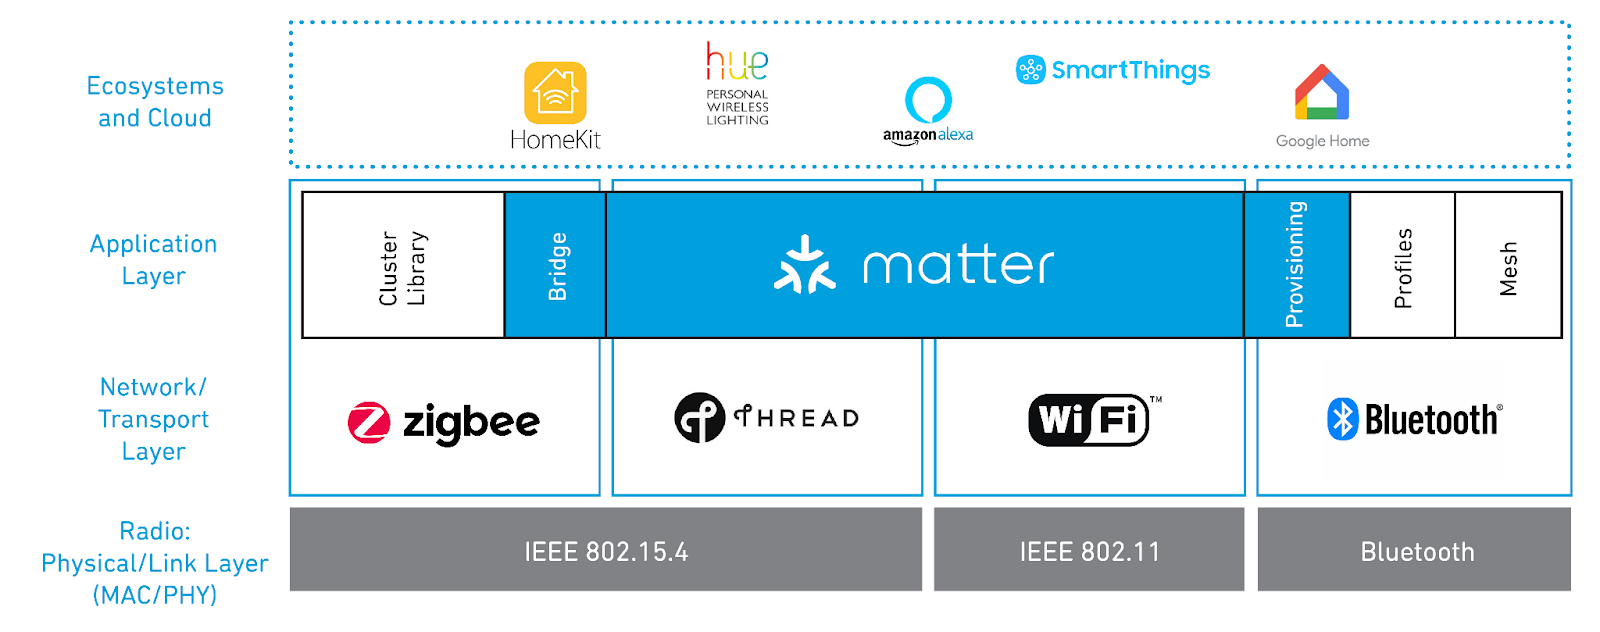
\includegraphics[width=0.9\textwidth]{DescricaoProcesso/Figuras/matter_big_arc.png}
  \caption{Arquitetura do \textit{Matter} como camada de aplicação.}
  \label{fig:matter-layer}
\end{figure}

Como descrito em \cite{matter_spec}, o protocolo Matter garante interoperabilidade entre diferentes dispositivos.

\subsection{Interface de Usuário}

A interface de usuário conecta pessoas e sistema, permitindo controle e monitoramento:

\begin{itemize}
    \item \textbf{Aplicativos Móveis e Web}: Acesso em qualquer lugar, visualização de histórico, criação de cenários e recebimento de notificações.
    \item \textbf{Painéis Físicos}: Telas sensíveis ao toque instaladas nas paredes, facilitando ajustes rápidos.
    \item \textbf{Assistentes Virtuais de Voz}: Google Assistant, Alexa, Siri, oferecendo controle sem a necessidade de interfaces gráficas.
\end{itemize}

Com o \textit{Matter}, a experiência do usuário é aprimorada, pois um único aplicativo ou assistente pode controlar dispositivos de diferentes marcas.

\subsection{Serviços em Nuvem e Análise de Dados}

A nuvem possibilita armazenamento histórico, análise avançada e integração com serviços externos:

\begin{itemize}
    \item \textbf{Análise Preditiva}: Antecipar consumos futuros, otimizar uso de energia.
    \item \textbf{Tarifas Dinâmicas}: Ajustar consumo conforme variação de preços de energia.
    \item \textbf{Manutenção Preditiva}: Identificar falhas iminentes em equipamentos.
\end{itemize}

A nuvem também permite acesso remoto, controle global e integração de APIs de terceiros, ampliando a funcionalidade do sistema.

\subsection{Segurança e Privacidade}

A crescente conectividade na automação residencial traz desafios que vão além de questões técnicas, abrangendo também a proteção de dados e o cumprimento de leis como a Lei Geral de Proteção de Dados (LGPD) no Brasil e o Regulamento Geral sobre a Proteção de Dados (GDPR) na União Europeia. Nesse contexto, é indispensável adotar medidas de segurança cibernética e garantir a privacidade dos moradores, protegendo suas informações pessoais e rotinas. O sistema deve incorporar, desde a fase de projeto, uma abordagem de \textit{Privacy by Design}, assegurando que mecanismos de proteção e conformidade estejam integrados às suas camadas mais básicas.

As principais práticas incluem:

- \textbf{Criptografia}: Todos os dados sensíveis coletados, transmitidos e armazenados devem ser protegidos por criptografia robusta, tornando-os ilegíveis a terceiros não autorizados. Assim, mesmo em caso de interceptação do tráfego de rede, informações pessoais não serão expostas, cumprindo princípios de segurança e confidencialidade exigidos pela LGPD.

- \textbf{Autenticação de Dispositivos}: Garantir que apenas dispositivos autenticados e confiáveis acessem a rede doméstica. Isso envolve a implementação de certificados digitais, chaves criptográficas ou outros métodos de autenticação forte. A restrição de acesso a dispositivos não autorizados previne usos indevidos das informações e atende aos princípios de prevenção e segurança previstos na LGPD.

- \textbf{Atualizações Seguras}: Manter o firmware dos dispositivos atualizado, corrigindo vulnerabilidades e garantindo um nível adequado de segurança contínua. O processo de atualização deve ser autenticado e seguro, impedindo que versões maliciosas sejam instaladas. Essa prática previne incidentes que possam expor dados pessoais e assegura a conformidade com a LGPD, pois reduz o risco de violações de segurança.

A privacidade é igualmente crítica. Dados sobre hábitos e rotinas dos moradores, bem como informações sobre ocupação da residência, uso de dispositivos específicos e preferências pessoais, devem ser armazenados e processados de modo a garantir o respeito à LGPD. Isso significa adotar princípios como minimização da coleta de dados (coletar apenas o indispensável para a finalidade proposta), consentimento informado dos usuários, transparência sobre como e por que os dados são usados e possibilidade de exclusão dos mesmos mediante solicitação. Além disso, todas as práticas de tratamento de dados devem estar documentadas e auditáveis, para comprovação de conformidade quando necessário.

\subsection{Integração com Outros Sistemas}

A automação residencial não funciona isoladamente. Ela pode integrar-se a sistemas de segurança, entretenimento, eletrodomésticos inteligentes e geração distribuída de energia, formando um ecossistema mais rico e funcional. Por exemplo, o sistema pode ajustar o uso de energia com base na produção solar local ou desativar determinados dispositivos ao detectar que a casa está vazia. No entanto, ao integrar múltiplos sistemas e plataformas, a complexidade na gestão dos dados aumenta. Nesse cenário, é fundamental garantir que todos os serviços externos cumpram também as normas de privacidade e segurança, incluindo a LGPD, mantendo assim a coerência e a proteção dos dados em todo o ecossistema.

\subsection{Escalabilidade e Flexibilidade}

A capacidade de crescer e se adaptar às mudanças é vital. Um sistema de automação residencial deve suportar a adição de novos dispositivos, tecnologias e serviços sem exigir reestruturações complexas. O uso de padrões abertos, como o \textit{Matter}, fortalece a escalabilidade e flexibilidade, garantindo que o sistema possa evoluir junto com o usuário e o mercado. Neste contexto, qualquer expansão deve manter o mesmo nível de conformidade com a LGPD, ampliando as práticas de segurança e privacidade para acomodar novos fluxos de dados, dispositivos e funcionalidades sem comprometer a proteção das informações pessoais.

\subsection{Instrumentação do Processo}

A instrumentação do processo envolve a seleção, instalação e configuração de sensores, atuadores e controladores. Esse cuidado na instrumentação não apenas assegura a qualidade dos dados e a efetividade das ações executadas, como também garante que o tratamento das informações coletadas obedeça aos princípios da LGPD e demais normas de proteção de dados. Para isso, alguns cuidados adicionais devem ser tomados:

- \textbf{Seleção de Hardware}: Além de atender às faixas de operação e às especificações técnicas, é importante escolher sensores e atuadores de fabricantes comprometidos com práticas adequadas de segurança e privacidade. O hardware deve permitir a implementação de criptografia, controle de acesso e atualizações seguras. Dispositivos que já seguem padrões abertos e oferecem mecanismos de proteção de dados facilitam a conformidade legal.

- \textbf{Topologia da Rede}: Ao projetar a rede, deve-se garantir cobertura de sinal, minimizar interferências e assegurar redundância em redes \textit{mesh}. Além da confiabilidade técnica, a topologia deve permitir segmentação da rede, isolando dispositivos críticos daqueles com maior risco de vulnerabilidades. Essa separação física ou lógica dificulta acessos não autorizados a dados sensíveis, contribuindo para a privacidade e segurança dos moradores.

- \textbf{Integração Elétrica}: A correta instalação elétrica, observando segurança, aterramento, fusíveis e normas técnicas, assegura não apenas o bom funcionamento dos componentes, mas também evita falhas que possam comprometer a segurança das informações. Curto-circuitos ou picos de tensão inesperados podem afetar módulos de segurança, chaves criptográficas ou até mesmo corromper dados sensíveis.

- \textbf{Provisionamento de Dispositivos}: A configuração inicial dos endereços, chaves de segurança e rotinas de atualização deve ser realizada de forma segura, garantindo que o dispositivo só seja controlado por usuários autorizados. Além disso, políticas de senhas fortes, autenticação de dois fatores e gestão de chaves criptográficas são práticas recomendadas. Essa etapa é essencial para assegurar conformidade com a LGPD, já que uma falha na configuração inicial pode resultar em acesso indevido a dados pessoais, comprometendo a privacidade dos moradores.

Em suma, a instrumentação não é apenas um aspecto técnico; ela é o alicerce para a proteção dos dados, a manutenção da segurança e o respeito à privacidade. Ao combinar boas práticas de engenharia com requisitos legais, o sistema de automação residencial pode operar de forma confiável, eficiente e em total conformidade com a LGPD e outras normas de proteção de dados.

\section{Monitoramento Energético}
\label{sec:monitoramento_energetico}

O monitoramento energético é um elemento central para a compreensão aprofundada do uso de recursos em um ambiente residencial automatizado. Mais do que simplesmente quantificar o consumo de eletricidade, o monitoramento energético permite revelar padrões, prever demandas futuras, identificar ineficiências e propor intervenções corretivas ou preventivas. Ao integrar dados provenientes de diversos sensores — incluindo aqueles dedicados à medição de corrente e tensão em circuitos específicos, bem como às tomadas e equipamentos inteligentes —, o sistema obtém uma visão holística do comportamento energético da residência.

Abaixo, são detalhadas as principais etapas e aspectos relacionados ao monitoramento energético, com especial ênfase na análise de dados, privacidade, conformidade com a LGPD, aplicações práticas e o uso de técnicas de controle estatístico de processo.
\subsection{Coleta e Organização dos Dados}

A primeira etapa do monitoramento energético consiste na coleta sistemática de dados relativos ao consumo de eletricidade em diferentes pontos da residência. Esses dados podem ser obtidos por meio de:

\begin{itemize}
    \item \textbf{Sensores de Consumo em Tempo Real}: Dispositivos que medem corrente e tensão, permitindo o cálculo instantâneo da potência e energia consumidas em circuitos específicos ou em eletrodomésticos individuais.
    \item \textbf{Tomadas e Disjuntores Inteligentes}: Elementos capazes de registrar o uso energético de um aparelho conectado, bem como ligar ou desligar o fornecimento conforme instruções do controlador.
    \item \textbf{Medição Global da Residência}: Sensores posicionados no quadro elétrico principal, fornecendo uma visão macro do consumo, contra a qual se podem comparar dados mais granulares para identificar fontes de ineficiência.
\end{itemize}

A coleta contínua gera um grande volume de dados. Para lidar com isso, é essencial adotar uma infraestrutura de armazenamento e processamento robusta. Uma opção comum é o uso de um \textbf{NAS (Network Attached Storage)}, um dispositivo de armazenamento conectado à rede local que fornece espaço centralizado e seguro para arquivamento dos dados. O NAS permite acesso controlado, backup automático e fácil ampliação da capacidade de armazenamento. Além disso, a utilização de sistemas em nuvem, servidores locais ou híbridos pode complementar o NAS, garantindo resiliência, segurança e acessibilidade dos dados.

Em qualquer cenário, devem-se implementar mecanismos de segurança (criptografia, autenticação forte) e compressão/normalização para facilitar o processamento posterior.

\subsection{Pré-Processamento, Qualidade dos Dados e Controle Estatístico de Processo}

Antes de realizar análises avançadas, os dados coletados precisam passar por etapas de pré-processamento, incluindo:

\begin{itemize}
    \item \textbf{Limpeza de Dados}: Remoção de leituras espúrias, tratamento de valores faltantes e correção de discrepâncias causadas por ruído elétrico ou falhas de comunicação.
    \item \textbf{Agregação e Granularidade}: Ajuste da escala temporal (por exemplo, sumarizar leituras segundo a segundo, minuto a minuto ou hora a hora) e espacial (agrupando dados por cômodo, circuito ou categoria de aparelho).
    \item \textbf{Normalização e Padronização}: Transformação dos dados em escalas comparáveis, permitindo análises consistentes entre diferentes pontos de medição ou períodos.
\end{itemize}

Um conjunto de dados bem pré-processado é mais coerente, confiável e adequado à aplicação de técnicas de análise estatística, aprendizado de máquina e modelagem preditiva.

Nesse contexto, o \textbf{Controle Estatístico de Processo (CEP)} pode ser aplicado ao monitoramento energético como uma ferramenta para acompanhar a variabilidade do consumo ao longo do tempo. Oriundo do domínio da qualidade industrial, o CEP utiliza gráficos de controle e limites estatísticos para distinguir variações normais de anomalias. Aplicado à automação residencial, o CEP permite:

\begin{itemize}
    \item \textbf{Estabelecer Faixas Normais de Operação}: Determinar limites superiores e inferiores para o consumo esperado, considerando padrões históricos e características da residência.
    \item \textbf{Detecção Precoce de Anomalias}: Identificar rapidamente desvios significativos, como um aumento inesperado no consumo de um aparelho, indicando falha ou uso indevido.
    \item \textbf{Monitoramento Contínuo}: Acompanhar a evolução do consumo ao longo do tempo, avaliando se as mudanças implementadas (como troca de um equipamento ou ajuste nas rotinas) resultam em maior eficiência.
\end{itemize}

O CEP atua como um complemento às técnicas de análise mais complexas, ajudando a manter o sistema dentro de parâmetros normais e fornecendo bases para intervenções pontuais.
\subsection{Análise Estatística e Inteligência Artificial}
Com dados limpos e estruturados, bem como limites estatísticos definidos pelo CEP, torna-se possível aplicar uma variedade de técnicas analíticas para extrair valor significativo:

\begin{itemize}
    \item \textbf{Estatística Descritiva}: Cálculo de médias, medianas, desvios-padrão e percentis para caracterizar o perfil de consumo energético ao longo do tempo.
    \item \textbf{Detecção de Anomalias Avançada}: Em conjunto com o CEP, métodos de aprendizado de máquina podem reconhecer padrões não lineares, detectando anomalias sutis que escapariam a métodos estatísticos convencionais.
    \item \textbf{Análise de Correlação e Causalidade}: Estabelecer relações entre o consumo energético e outras variáveis (temperatura, ocupação, eventos externos).
    \item \textbf{Modelagem Preditiva}: Uso de algoritmos de aprendizado supervisionado ou não supervisionado para prever demandas futuras, ajustar parâmetros de controle em tempo real e recomendar intervenções.
    \item \textbf{Clusterização de Perfis de Consumo}: Agrupamento de padrões de uso semelhantes, auxiliando na identificação de zonas energéticas e na otimização personalizada do sistema.
\end{itemize}

A inteligência artificial, combinada ao CEP, amplia as capacidades do sistema, tornando-o mais adaptativo e robusto. Isso resulta em ajustes proativos na operação da residência, reduzindo custos, melhorando o conforto e minimizando impactos ambientais.

\subsection{Privacidade, LGPD e Proteção dos Dados Energéticos}

As informações sobre consumo energético podem revelar hábitos, presença, rotinas e preferências dos moradores. Como tais dados podem ser considerados pessoais ou sensíveis segundo a LGPD, devem ser tratados com o mesmo rigor aplicado a outras informações coletadas:

\begin{itemize}
    \item \textbf{Minimização de Dados}: Coletar apenas o nível de detalhe necessário.  
    \item \textbf{Anonimização e Pseudonimização}: Remover ou mascarar informações identificadoras.
    \item \textbf{Consentimento e Transparência}: Explicar claramente aos moradores como, por que e por quanto tempo os dados serão coletados, analisados e armazenados.
    \item \textbf{Segurança da Informação}: Aplicar criptografia ponta a ponta, autenticação robusta e isolamento de redes.
    \item \textbf{Auditorias e Responsabilização}: Manter registros sobre o tratamento de dados, comprovando conformidade com a LGPD em caso de inspeções.
\end{itemize}

Ao equilibrar análise de dados avançada, CEP e privacidade, o monitoramento energético torna-se não apenas um recurso valioso, mas também uma solução respeitosa aos direitos e expectativas dos usuários.

\subsection{Integração com Outros Sistemas e Evolução Contínua}

O monitoramento energético não existe isoladamente. Ao integrar-se com controladores, sistemas de climatização, iluminação e segurança, bem como com serviços em nuvem e APIs externas, o sistema pode ajustar em tempo real o uso de energia conforme necessidades, demandas e condições externas.

Com a aplicação do CEP, é possível identificar se as integrações e ajustes recomendados estão mantendo o consumo dentro dos limites estatísticos esperados ou se intervenções adicionais são necessárias. Conforme novos dispositivos e tecnologias surgem, a arquitetura flexível e o uso de padrões abertos, como o \textit{Matter}, asseguram que o sistema seja escalável e possa incorporar inovações sem comprometer a segurança, a privacidade ou a qualidade da análise de dados.
\subsection{Benefícios Práticos e Responsabilidade Social}

Quando bem implementado, o monitoramento energético, aliado ao CEP e à análise de dados, traz diversos benefícios:

\begin{itemize}
    \item \textbf{Eficiência e Economia}: Redução de custos com energia elétrica por meio da identificação de desperdícios e ajustes estratégicos.
    \item \textbf{Conforto e Qualidade de Vida}: Ajustes automáticos de parâmetros ambientais conforme preferências e necessidades, sem intervenção manual constante.
    \item \textbf{Sustentabilidade}: Otimização do uso de energia, priorizando fontes renováveis e reduzindo a pegada de carbono.
    \item \textbf{Tomada de Decisão Baseada em Evidências}: Dados claros, validados e dentro de parâmetros estatísticos auxiliares guiam melhorias contínuas e embasadas em fatos.
\end{itemize}

A responsabilidade social emerge ao assegurar que tais benefícios sejam obtidos sem invadir a privacidade ou violar direitos fundamentais. A conformidade com a LGPD, o uso ético da análise de dados e a adoção de CEP garantem que a tecnologia melhore a vida dos moradores, mantendo a confiança e a proteção das informações pessoais.
Em síntese, o monitoramento energético aplicado a um sistema de automação residencial, quando embasado em um arcabouço analítico sólido, conformidade regulatória, uso de CEP e cuidado com a privacidade, transcende a mera coleta de dados. Ele estabelece um processo contínuo de aprendizado, ajuste e otimização que beneficia usuários, meio ambiente e sociedade em geral.  
\bibliography{Monografia}%,library}
\chapter{Metodologia}

Neste capítulo, são detalhadas as etapas metodológicas adotadas no desenvolvimento do sistema inteligente para monitoramento e previsão do consumo de energia residencial. A abordagem foi projetada para atender aos objetivos do projeto, combinando análise técnica, desenvolvimento de soluções e validação experimental. Os procedimentos descritos têm como objetivo garantir a reprodução, escalabilidade e eficácia do sistema proposto, contribuindo para o avanço na área de automação e eficiência energética.

\section{Pesquisa e Análise de Tecnologias Existentes}

A fase inicial do projeto consistiu na identificação e análise das tecnologias disponíveis no mercado para o monitoramento de consumo energético em residências. Esta etapa foi guiada por uma revisão bibliográfica abrangente e um estudo comparativo das soluções existentes, considerando os seguintes critérios:

\begin{itemize}
    \item \textbf{Compatibilidade com infraestruturas residenciais convencionais}: Tecnologias que não exigem modificações estruturais significativas, como sensores de fácil instalação e dispositivos autônomos.
    \item \textbf{Eficiência técnica}: Precisão na coleta de dados, robustez e confiabilidade das medições.
    \item \textbf{Interoperabilidade}: Capacidade de integração com diferentes sistemas e protocolos, como Wi-Fi, Zigbee e Bluetooth Low Energy.
    \item \textbf{Custo-benefício}: Viabilidade econômica para implementação em larga escala.
\end{itemize}

A análise resultou na seleção de componentes que atendem aos requisitos do projeto. Foi escolhida a linha de tomadas \textit{Tuya Smart Wi-Fi}, cuja modularidade permite fácil instalação em diversos locais, utilizando a metodologia \textit{plug and play}. Estas tomadas oferecem integração com a plataforma \textit{Tuya Cloud} e suas APIs, garantindo flexibilidade e escalabilidade.

\section{Desenvolvimento do Protótipo}

Com base nas tecnologias identificadas, foi desenvolvido um protótipo funcional que integra hardware e software para monitoramento e previsão de consumo energético. O desenvolvimento seguiu as seguintes etapas:

\subsection{Seleção e Configuração de Sensores}

As tomadas \textit{Tuya Smart Wi-Fi} foram configuradas para monitorar o consumo energético em tempo real. Estes dispositivos enviam os dados para a plataforma \textit{Tuya Cloud}, de onde são acessados por meio de APIs.

\subsection{Desenvolvimento do Sistema de Controle}

O sistema de controle foi desenvolvido utilizando as APIs fornecidas pela \textit{Tuya Cloud}, permitindo a comunicação entre as tomadas e o sistema central. O controlador é responsável por:

\begin{itemize}
    \item Receber e processar os dados coletados pelas tomadas.
    \item Aplicar algoritmos de análise e previsão de consumo.
    \item Integrar os dados a uma interface de visualização desenvolvida especificamente para o projeto.
\end{itemize}

\subsection{Desenvolvimento da Interface de Visualização}

A interface de monitoramento foi desenvolvida pelo autor do trabalho utilizando linguagens de programação voltadas para desenvolvimento web e visualização de dados. Esta interface exibe de forma intuitiva os padrões de consumo energético, permitindo que os usuários identifiquem desperdícios e ajustem seu comportamento para otimizar o uso de energia.

\section{Implementação de Algoritmos de Processamento e Previsão}

Para o tratamento dos dados coletados, foram desenvolvidos e implementados algoritmos específicos, detalhados a seguir:

\subsection{Pré-processamento dos Dados}

Os dados brutos coletados pelas tomadas passaram por etapas de limpeza e normalização, eliminando leituras espúrias e garantindo consistência nos resultados.

\subsection{Análise Estatística e Controle Estatístico de Processos (CEP)}

O CEP foi utilizado para identificar variações significativas no consumo energético, estabelecendo limites de controle e detectando anomalias. Esta abordagem foi complementada por métodos estatísticos descritivos para caracterizar os padrões de consumo.

\subsection{Previsão de Consumo com Inteligência Artificial}

Modelos de aprendizado de máquina foram treinados utilizando dados históricos para prever demandas futuras de energia. Técnicas como regressão linear e redes neurais foram aplicadas, visando maior precisão e adaptabilidade.

\section{Validação em Ambiente Real}

O protótipo foi testado em um ambiente residencial que não possuía infraestrutura prévia de automação. A validação envolveu:

\begin{itemize}
    \item \textbf{Avaliação de desempenho}: Testes para verificar a precisão das tomadas \textit{Tuya Smart Wi-Fi} e a eficiência dos algoritmos.
    \item \textbf{Usabilidade}: Análise da interface para garantir que usuários finais pudessem interpretar os dados facilmente.
    \item \textbf{Robustez}: Monitoramento contínuo em condições reais, avaliando a resiliência do sistema a falhas.
\end{itemize}

Os resultados dos testes foram documentados e utilizados para refinar o sistema, corrigindo inconsistências e melhorando sua eficiência.

\section{Viabilidade de Implementação em Larga Escala}

A análise de viabilidade considerou aspectos técnicos, econômicos e sociais, como:

\begin{itemize}
    \item \textbf{Custos de produção}: Avaliação dos investimentos necessários para replicação do sistema.
    \item \textbf{Benefícios econômicos}: Potencial de redução de custos para os usuários com base na diminuição do desperdício energético.
    \item \textbf{Impactos ambientais}: Contribuição para a sustentabilidade por meio do uso eficiente de energia.
    \item \textbf{Estratégias de adoção}: Identificação de barreiras e propostas para ampliar o alcance do sistema, como parcerias com fabricantes de dispositivos inteligentes.
\end{itemize}

\section{Resumo do Capítulo}

Este capítulo detalhou as etapas metodológicas seguidas no desenvolvimento do sistema inteligente para monitoramento e previsão de consumo de energia residencial. As etapas compreenderam a análise de tecnologias, desenvolvimento do protótipo utilizando as tomadas \textit{Tuya Smart Wi-Fi}, implementação de algoritmos avançados, validação experimental e estudo de viabilidade em larga escala. A abordagem proposta combina rigor técnico e aplicabilidade prática, destacando-se como uma solução promissora para o setor de automação residencial.
\chapter{Resultados}

Para a execução do projeto, algumas etapas de desenvolvimento tiveram de ser seguidas: familiarização com o sistema, estudo dos módulos envolvidos, leitura dos requisitos, elaboração de documento descrevendo todo o processo de implementação e relacionamento com os diversos módulos, implementação e testes.


\section{Atividades do Projeto}
\label{metodo3}

\section {Requisitos do Sistema}
\label{req}


\section{Desenvolvimeto e Implementação}

A Tabela \ref{tab:tabela} apresenta as atividades executadas.

\begin{table}
\centering
%Note os alinhamentos diferentes em cada coluna
\begin{tabular}{|c|r|l|}\hline
		Atividade 1 & aa  & ab  \\ 
					 & a & b \\ \hline
		Ativ. 2  & aa & ab \\			
					 &  a & b \\ \hline
		\end{tabular}
	\caption{Exemplo de tabela - Coloque toda informação sobre a tabela aqui}
	\label{tab:tabela}
\end{table}

\section{Testes}

\section{Análise dos Resultados}

Apresente os resultados sem adulterações e faça análises objetivas. Pense na melhor maneira de apresentar os resultados graficamente. Se os gráficos são difíceis de interpretar, talvez tabelas sejam uma forma melhor de apresentar resultados. Não apresente dados (gráficos e tabelas) se não há uma conclusão interessante a ser tirada. Lembre-se de ser conciso.

\emph{Não se esqueça das unidades!} Pense que \emph{a priori} todo número deve ter uma unidade. Não escreva as unidades em itálico (no ambiente matemático) e tome cuidado para diferenciar maiúsculas e minúsculas. Um exemplo é escrever $22$ [kN] e não $22 KN$ (Kelvin vezes Newton!).

Ao apresentar resultados experimentais, tome o cuidado para também apresentar o cálculo das incertezas sempre que forem significativas. Ao fazer conclusões, sempre considere se o tamanho da sua amostra é grande o suficiente do ponto de vista estatístico. Lembre que a média empírica $\hat{\mu}_X$ de $N$ observações independentes da variável $X_i$ possui variância
\[
\hat{\sigma}_{\mu}^2 = \frac{1}{N(N-1)} \sum_{i=1}^N (X_i-\hat{\mu}_X)^2
\enspace,
\]
onde se assume que as variáveis $X_i$ possuem uma mesma ditribuição e que essa distribuição possui segundo momento finito.


\section{Resumo do Capítulo}
\label{sec:resumoo4}
Tente não terminar de forma abrupta. Se for escrever algo aqui, não seja genérico!

\section{Formato, expressões matemáticas e o \LaTeX}

\subsection{O \LaTeX}

O {\LaTeX}  é o método preferencial de preparação de documentos para textos técnicos nas ciências exatas. O {\LaTeX} permite não só lidar com equações de uma forma mais prática que em editores de texto, mas também facilita a formatação de documentos e tem um desempenho marcadamente superior a editores de texto na preparação de documentos longos como monografias. 

Documentos em {\LaTeX} são escritos em um ou mais arquivos de texto com extensão .tex. Após a escrita, o .tex é \emph{compilado} para gerar arquivos nos formatos .pdf, .dvi ou .ps. Hoje há duas distribuições padrão para o \LaTeX. Sistemas Windows usam o {Mik\TeX} e sistemas Unix usam o \TeX Live. Além das distribuições, muitos usuários utilizam \emph{front-ends} que facilitam a edição do texto, a compilação e a instalação de pacotes. 

Os pacotes necessários para compilar o presente documento devem ser encontrados numa instalação completa dessas distribuições. Se tiver dificuldades com os pacotes, você pode instalá-los manualmente ou tentar alterar o código para usar versões antigas dos mesmos.

A compilação pode ser feita pelos comandos \textsf{latex} ou \textsf{pdflatex}, invocados pela linha de comando ou pelo \emph{front-end}. Note que será necessário empregar o comando \textbf{mais de uma vez} para que as referências cruzadas saiam corretas.

Como discutido na Seção \ref{sec:revisão}, uma ferramenta útil para gerenciar as citações em {\LaTeX} é o Bib\TeX. Para gerar uma lista bibliográfica a partir do arquivo .bib, este arquivo deve ser indicado no arquivo .tex. Em seguida devem-se executar os comandos \textsf{pdflatex}, \textsf{bibtex} e \textsf{pdflatex} novamente sempre usando o .tex como argumento. Note que os comandos são executados nesta ordem e de forma repetida para que as referências cruzadas sejam geradas corretamente.

Nesta seção você deve encontrar exemplos dos comandos mais usados em \LaTeX. Outros exemplos e manuais podem ser encontrados na internet com facilidade.

\subsection{Expressões Matemáticas}

Ao escrever expressões matemáticas, defina todas as variáveis antes de usá-las ou imediatamente depois da expressão. Deixar de fazê-lo torna seu texto \textbf{ilegível}. Segue um exemplo.

Seja o par $(a_1,a_2)\in \mathbb{R}^2$. Para $s\in\mathbb{C}$, definimos a função $f(s)$ como
\[%cria equações sem numeração
f(s)\triangleq \frac{a_1 s+a_2}{s^2+2\zeta\omega_n s+\omega_n^2}
\enspace,
\]
onde os escalares $\zeta,\omega_n>0$ são constantes.

Note que não foi necessário atribuir valores às variáveis neste momento. Repare também como devemos \textbf{usar pontuação} (vírgula) nas equações, tratando-as como parte da frase. Usamos o símbolo $\triangleq$ ou $:=$ para deixar explícito que se trata de uma definição. Ser claro nesse aspecto facilita o entendimento do leitor.

A equação acima não foi numerada porque não será citada no texto. Vejamos um exemplo com numeração.

A função $f(\cdot)$ possui um zero em $-a_2/a_1$ (ou $-\frac{a_2}{a_1}$) e, para $\zeta<1$, possui polos complexos $p_{1,2}$ dados por
\begin{equation}
\label{eq:polos}
p_{1,2}=\omega_n \left(-\zeta\pm j\sqrt{1-\zeta^2}\right)
\enspace.
\end{equation}
Agora podemos citar os polos dados pela Equação (\ref{eq:polos}) (aqui adotamos a convenção de citar sempre com o número entre parênteses precedido da palavra Equação). Note como usamos um comando especial na Equação \ref{eq:polos} para garantir o ajuste automático do tamanho dos parênteses.

Vejamos agora como criar equações alinhadas. Considere o sistema dinâmico dado pelas equações diferenciais:

\begin{align}
\dot{x}_1 & = \cos(x_2)\cdot\ln(1/x_1)+\tan(u) \label{eq:x1dot} \\
\dot{x}_2 & = e^{-x_1-x_2} \nonumber \\
& y  = \min\{x_1,x_2\}  \label{eq:saida}
\enspace,
\end{align}
onde $x(t)=[x_1(t) ~ x_2(t)]'$, $t>0$, é a variável de estado do sistema, $u(t)$ é o sinal de entrada e $y(t)$ é o sinal de saída do sistema. Note no .tex que o caracter de tabulação \textsf{\&} foi usado para indicar o ponto de alinhamento horizontal das equações. Além disso, para ilustrar o uso do \LaTeX, retiramos a numeração da segunda equação e citamos as equações separadamente.

Nas Equações (\ref{eq:x1dot}) e (\ref{eq:saida}), aparecem operadores como $\min$, $\ln$, $\cos$ e $\tan$. A convenção aqui é que \textbf{variáveis devem ser escritas em itálico e operadores não}. Por essa razão todas as expressões matemáticas devem ser escritas no ambiente matemático (entre cifrão) mesmo quando for possível usar texto comum. Isso garante a consistência das fontes utilizadas (nem sempre a fonte do ambiente matemático é a mesma fonte do texto). 

Para escrever matrizes, podemos fazer por exemplo:
\[
\sum_{n=0}^{\infty}z^{-n}\left[\begin{array}{cc}
\lambda & 1 \\
0 & \lambda
\end{array}\right]^n=
\left[\begin{array}{cc}
\frac{z}{z-\lambda} & \frac{z}{(z-\lambda)^2} \\
0 & \frac{z}{z-\lambda}
\end{array}\right]
,~\forall \lambda<|z|
\enspace.
\]

Para escrever uma expressão com múltiplos casos, podemos fazer, para um inteiro $N$ positivo,
\[
g[n]=
\left\{
\begin{array}{ll}
0,& \mbox{se }~ n\leq 0 \\
n,& \mbox{se }~ n=1,2,\ldots,N-1 \\
N,& \mbox{se }~ n\mod N = 0 \\
0,& \mbox{caso contrário}\enspace.
\end{array}
\right.
\]

\textbf{Nunca reaproveite símbolos} matemáticos, isto é, nunca use o mesmo símbolo para designar variáveis diferentes.

Para um exemplo com múltiplas linhas de expressão matemática: tem-se que, para $a\neq 0$,

\begin{equation}
\begin{split}
ax^2+bx+c &= 0 \\
& \Rightarrow a(x^2+bx/a+c/a) =0 \Rightarrow a((x+b/(2a))^2+c/a-b^2/(4a^2))=0  \\
& \Rightarrow (x+b/(2a))^2=(b^2-4ac)/(4a^2) \\
& \Rightarrow (x+b/(2a))=\pm\sqrt{b^2-4ac}/(2a) \\
& \Rightarrow x=\frac{-b\pm\sqrt{b^2-4ac}}{2a}
\enspace.
\end{split}
\end{equation}

Note a argumentação lógica aqui. Não estamos dizendo que o valor de $x$ é dado pela última linha. Estamos dizendo que a hipótese da primeira linha juntamente com a hipótese $a\neq 0$ implicam os referidos valores de $x$. \textbf{Um erro comum dos alunos ao escrever é não distinguir a veracidade das implicações com a veracidade das hipóteses}.

\clearpage
\chapter{Conclusões}

Novamente, este será um dos trechos que o leitor experiente lerá antes de decidir se vale a pena ler o texto integral. Seja convincente.

\section{Considerações Finais}

Reitere o que de mais importante foi feito, qual era o objetivo inicial e qual o resultado obtido. Se houve requisitos ou especificações de projeto, discuta se foram atingidos. Se os resultados não foram conclusivos ou contrariam o que se esperava, seja honesto e diga-o explicitamente. Busque explicar os insucessos com argumentos sólidos e plausíveis. 

\section{Propostas de Continuidade}

Se houve questões ainda não respondidas ou resultados insatisfatórios, aponte direções de continuação.

\clearpage


\addcontentsline{toc}{chapter}{Referências Bibliográficas}
\renewcommand{\bibname}{Referências Bibliográficas}

%\bibliographystyle{abntex2-alf} %para norma ABNT no sistema autor-data
\bibliographystyle{abntex2-num}
\begin{small}
\bibliography{ListadeReferencias}%,library}
%% Monografia para Projeto de Fim de Curso - Exemplo no LaTeX
%-----------------------------------------------------------


%---------------Inicialização de pacotes--------------------

\documentclass[12pt,a4paper,notitlepage,twoside]{book}


\usepackage{graphicx}
\usepackage[utf8]{inputenc}
%\usepackage[latin1]{inputenc} %%pode ser necessário trocar a codificação em sistemas Windows
\usepackage[brazil]{babel}		%%pode ser necessário trocar o pacote de línguas em algumas distribuições LateX
%\usepackage[portuguese]{babel}
\usepackage[T1]{fontenc}
\usepackage{amsmath,amssymb}
\usepackage{amsthm,amsfonts}
\usepackage{color}
\usepackage[colorlinks]{hyperref}
\usepackage{abntex2abrev}
%\usepackage[alf]{abntex2cite} %se você quiser seguir as normas ABNT no sistema autor-data
%\usepackage[num]{abntex2cite} %se você quiser seguir as normas ABNT no sistema numérico
\usepackage{setspace}
\usepackage[toc,page]{appendix}

%Definindo fonte Times (Use os pacotes obsoletos se não conseguir instalar os atualizados)
%\usepackage{times}     %Pacote de fontes obsoleto, apenas texto
%usepackage{mathptmx}  %Pacote de fontes obsoleto, texto e símbolos matemáticos
%\usepackage{newtxtext,newtxmath}  %Pacotes de fontes mais recentes

\usepackage[a4paper,top=30mm,bottom=30mm,inner=30mm,outer=25mm,headheight=7mm,headsep=6mm,footskip=7mm]{geometry}
\usepackage{enumerate}

\makeindex

%\singlespacing   %%espaçamento simples
%\onehalfspacing
%\setstretch{1.03} %%um pouco melhor que espaçamento simples
\linespread{1.25} %corresponde ao espaçamento 1.5 do MS Word

%---------------Início do documento-------------------------

\begin{document}

\include{Capa/capa}

\pagenumbering{roman}
\include{Resumo/Resumo}
\include{Resumo/Abstract}
\include{Agradecimentos/Agradecimentos}
\include{TabelaConteudo/TabelaConteudo}
\include{ListaFiguras/ListaFiguras}
\include{ListaTabelas/ListaTabelas}

\pagenumbering{arabic}
\setcounter{page}{1}
\include{Introducao/Introducao}
\include{DescricaoProcesso/DescricaoProcesso}
\include{Metodologia/Metodologia}
\include{Resultados/Resultados}
\include{Conclusao/Conclusao}

\addcontentsline{toc}{chapter}{Referências Bibliográficas}
\renewcommand{\bibname}{Referências Bibliográficas}

%\bibliographystyle{abntex2-alf} %para norma ABNT no sistema autor-data
\bibliographystyle{abntex2-num}
\begin{small}
\bibliography{ListadeReferencias}%,library}
%\input{Monografia.bbl}
\end{small}

%\begin{appendices}
\appendix
\include{Apendices/ApendiceA}
\include{Apendices/ApendiceB}
%\end{appendices}

\end{document}

%---------------Fim do documento----------------------------
\end{small}

%\begin{appendices}
\appendix
\chapter{O que ficou para depois}

Inclua aqui informações que não sejam tão relevantes para o entendimento do projeto mas que ainda sejam importantes para documentá-lo. 
\chapter{O que mais faltou}

Inclua aqui informações que não sejam tão relevantes para o entendimento do projeto mas que ainda sejam importantes para documentá-lo. 
%\end{appendices}

\end{document}

%---------------Fim do documento----------------------------
\end{small}

%\begin{appendices}
\appendix
\chapter{O que ficou para depois}

Inclua aqui informações que não sejam tão relevantes para o entendimento do projeto mas que ainda sejam importantes para documentá-lo. 
\chapter{O que mais faltou}

Inclua aqui informações que não sejam tão relevantes para o entendimento do projeto mas que ainda sejam importantes para documentá-lo. 
%\end{appendices}

\end{document}

%---------------Fim do documento----------------------------
\end{small}

%\begin{appendices}
\appendix
\chapter{O que ficou para depois}

Inclua aqui informações que não sejam tão relevantes para o entendimento do projeto mas que ainda sejam importantes para documentá-lo. 
\chapter{O que mais faltou}

Inclua aqui informações que não sejam tão relevantes para o entendimento do projeto mas que ainda sejam importantes para documentá-lo. 
%\end{appendices}

\bibliography{ListadeReferencias}%,library}
\end{document}
%---------------Fim do documento----------------------------